 \documentclass[11pt]{article}
 
\def\shownotes{1}
\def\blinded{0}


\usepackage[top=3cm, bottom=3cm, left=2cm, right=2cm]{geometry}      % [top=2cm, bottom=2cm, left=2cm, right=2cm]
\geometry{letterpaper}                   % ... or a4paper or a5paper or ...
%\geometry{landscape}                % Activate for for rotated page geometry
%\usepackage[parfill]{parskip}
\usepackage{graphicx}
\usepackage{amssymb, amsmath, amsfonts}
\usepackage{amsthm}
\usepackage{enumerate}
\usepackage{hyperref}
\usepackage{xspace}
\usepackage{graphicx}
\usepackage{latexsym}
\usepackage{color}
\usepackage{framed}
\usepackage{algpseudocode}

\mathchardef\mhyphen="2D

\newcommand{\secref}[1]{\mbox{Section~\ref{#1}}}
\newcommand{\subsecref}[1]{\mbox{Subsection~\ref{#1}}}
\newcommand{\apref}[1]{\mbox{Appendix~\ref{#1}}}
\newcommand{\thref}[1]{\mbox{Theorem~\ref{#1}}}
\newcommand{\exref}[1]{\mbox{Example~\ref{#1}}}
\newcommand{\defref}[1]{\mbox{Definition~\ref{#1}}}
\newcommand{\corref}[1]{\mbox{Corollary~\ref{#1}}}
\newcommand{\lemref}[1]{\mbox{Lemma~\ref{#1}}}
\newcommand{\assref}[1]{\mbox{Assumption~\ref{#1}}}
\newcommand{\probref}[1]{\mbox{Problem~\ref{#1}}}
\newcommand{\clref}[1]{\mbox{Claim~\ref{#1}}}
\newcommand{\propref}[1]{\mbox{Proposition~\ref{#1}}}
\newcommand{\remref}[1]{\mbox{Remark~\ref{#1}}}
\newcommand{\consref}[1]{\mbox{Construction~\ref{#1}}}
\newcommand{\figref}[1]{\mbox{Figure~\ref{#1}}}
\DeclareMathOperator*{\expe}{\mathbb{E}}
\DeclareMathOperator*{\var}{\text{Var}}


\newcommand{\class}[1]{{\ensuremath{\mathsf{#1}}}}
\newcommand{\gen}{\ensuremath{\class{Gen}}\xspace}
\newcommand{\rep}{\ensuremath{\class{Rep}}\xspace}
\newcommand{\sketch}{\ensuremath{\class{SS}}\xspace}
\newcommand{\rec}{\ensuremath{\class{Rec}}\xspace}
\newcommand{\enc}{\ensuremath{\class{Enc}}\xspace}
\newcommand{\dec}{\ensuremath{\class{Dec}}\xspace}
\newcommand{\prg}{\ensuremath{\class{prg}}\xspace}
\newcommand{\crust}{\ensuremath{\class{Crust}}\xspace}
\newcommand{\inter}{\ensuremath{\class{Inter}}\xspace}
\newcommand{\zo}{\ensuremath{\{0, 1\}}}
\newcommand{\vect}[1]{\ensuremath{\mathbf{#1}}}
\newcommand{\zq}{\ensuremath{\mathbb{Z}_q}}
\newcommand{\Fq}{\ensuremath{\mathbb{F}_q}}
\newcommand{\sample}{\ensuremath{\class{Sample}}\xspace}
\newcommand{\neigh}{\ensuremath{\class{Neigh}}\xspace}
\newcommand{\dis}{\ensuremath{\mathsf{dis}}}
\newcommand{\decode}{\ensuremath{\mathsf{Decode}}}
\newcommand{\guess}{\mathsf{guess}}


\newcommand{\A}{\mathcal{A}}


\newcommand{\metric}{\ensuremath{\mathtt{Metric}}\xspace}
\newcommand{\hill}{\ensuremath{\mathtt{HILL}}\xspace}
\newcommand{\hillrlx}{\ensuremath{\mathtt{HILL\mhyphen rlx}}\xspace}
\newcommand{\yao}{\ensuremath{\mathtt{Yao}}\xspace}
\newcommand{\unp}{\ensuremath{\mathtt{unp}}\xspace}
\newcommand{\unprlx}{\ensuremath{\mathtt{unp\mhyphen rlx}}\xspace}
\newcommand{\metricstar}{\ensuremath{\mathtt{Metric}^*}\xspace}
\newcommand{\metricd}{\ensuremath{\mathtt{Metric}^*\mathtt{-d}}\xspace}
\newcommand{\hillstar}{\ensuremath{\mathtt{HILL}^*}\xspace}
\newcommand{\hillprime}{\ensuremath{\mathtt{HILL'}}\xspace}
\newcommand{\metricprime}{\ensuremath{\mathtt{Metric'}}\xspace}
\newcommand{\metricprimestar}{\ensuremath{\mathtt{Metric'}^*}\xspace}
\newcommand{\hillprimestar}{\ensuremath{\mathtt{HILL'}^*}\xspace}
\newcommand{\poly}{\ensuremath{\mathtt{poly}}\xspace}
\newcommand{\rank}{\ensuremath{\mathtt{rank}}\xspace}
\newcommand{\ngl}{\ensuremath{\mathtt{ngl}}\xspace}
\newcommand{\Hoo}{\mathrm{H}_\infty}
\newcommand{\Hav}{\tilde{\mathrm{H}}_\infty}
\newcommand{\Hfuzz}{\mathrm{H}^{\mathtt{fuzz}}_{t,\infty}}
\newcommand{\Huse}{\mathrm{H}_{\mathtt{usable}}}
\newcommand{\Dom}{\mathsl{Dom}}
\newcommand{\Range}{\mathsl{Rng}}
\newcommand{\Keys}{\mathsl{Keys}}
\def\col{\mathrm{Col}}

\newcommand{\ddetbin}{\ensuremath{\mathcal{D}^{det,\{0,1\}}}}
\newcommand{\drandbin}{\ensuremath{\mathcal{D}^{rand,\{0,1\}}}}
\newcommand{\ddetrange}{\ensuremath{\mathcal{D}^{det,[0,1]}}}
\newcommand{\drandrange}{\ensuremath{\mathcal{D}^{rand,[0,1]}}}

\newcommand{\expinfo}{\ensuremath{\mathcal{E}}}
\newcommand{\ext}{\ensuremath{\mathtt{ext}}}
\newcommand{\cext}{\ensuremath{\mathtt{cext}}}
\newcommand{\rext}{\ensuremath{\mathtt{rext}}}
\newcommand{\cons}{\ensuremath{\mathtt{cons}}}
\newcommand{\decons}{\ensuremath{\mathtt{decons}}}


\newcommand{\lwe}{\class{LWE}}
\newcommand{\LWE}{\class{LWE}}
\newcommand{\distLWE}{\ensuremath{\class{dist\mbox{-}LWE}}}

\newtheorem{theorem}{Theorem}[section]
\newtheorem{lemma}[theorem]{Lemma}
\newtheorem{proposition}[theorem]{Proposition}
\newtheorem{corollary}[theorem]{Corollary}
\newtheorem{definition}[theorem]{Definition}
\newtheorem{assumption}[theorem]{Assumption}
\newtheorem{claim}[theorem]{Claim}
\newtheorem{problem}[theorem]{Problem}
\newtheorem{construction}[theorem]{Construction}

\newcounter{ctr}
\newcounter{savectr}
\newcounter{ectr}

\newenvironment{newitemize}{%
\begin{list}{\mbox{}\hspace{5pt}$\bullet$\hfill}{\labelwidth=15pt%
\labelsep=5pt \leftmargin=20pt \topsep=3pt%
\setlength{\listparindent}{\saveparindent}%
\setlength{\parsep}{\saveparskip}%
\setlength{\itemsep}{3pt} }}{\end{list}}


\newenvironment{newenum}{%
\begin{list}{{\rm (\arabic{ctr})}\hfill}{\usecounter{ctr} \labelwidth=17pt%
\labelsep=5pt \leftmargin=22pt \topsep=3pt%
\setlength{\listparindent}{\saveparindent}%
\setlength{\parsep}{\saveparskip}%
\setlength{\itemsep}{2pt} }}{\end{list}}

\newenvironment{tiret}{%
\begin{list}{\hspace{2pt}\rule[0.5ex]{6pt}{1pt}\hfill}{\labelwidth=15pt%
\labelsep=3pt \leftmargin=22pt \topsep=3pt%
\setlength{\listparindent}{\saveparindent}%
\setlength{\parsep}{\saveparskip}%
\setlength{\itemsep}{2pt}}}{\end{list}}


\newenvironment{blocklist}{\begin{list}{}{\labelwidth=0pt%
\labelsep=0pt \leftmargin=0pt \topsep=10pt%
\setlength{\listparindent}{\saveparindent}%
\setlength{\parsep}{\saveparskip}%
\setlength{\itemsep}{20pt}}}{\end{list}}

\newenvironment{blocklistindented}{\begin{list}{}{\labelwidth=0pt%
\labelsep=30pt \leftmargin=30pt\topsep=5pt%
\setlength{\listparindent}{\saveparindent}%
\setlength{\parsep}{\saveparskip}%
\setlength{\itemsep}{10pt}}}{\end{list}}

\newenvironment{onelist}{%
\begin{list}{{\rm (\arabic{ctr})}\hfill}{\usecounter{ctr} \labelwidth=18pt%
\labelsep=7pt \leftmargin=25pt \topsep=2pt%
\setlength{\listparindent}{\saveparindent}%
\setlength{\parsep}{\saveparskip}%
\setlength{\itemsep}{2pt} }}{\end{list}}

\newenvironment{twolist}{%
\begin{list}{{\rm (\arabic{ctr}.\arabic{ectr})}%
\hfill}{\usecounter{ectr} \labelwidth=26pt%
\labelsep=7pt \leftmargin=33pt \topsep=2pt%
\setlength{\listparindent}{\saveparindent}%
\setlength{\parsep}{\saveparskip}%
\setlength{\itemsep}{2pt} }}{\end{list}}

\newenvironment{centerlist}{%
\begin{list}{\mbox{}}{\labelwidth=0pt%
\labelsep=0pt \leftmargin=0pt \topsep=10pt%
\setlength{\listparindent}{\saveparindent}%
\setlength{\parsep}{\saveparskip}%
\setlength{\itemsep}{10pt} }}{\end{list}}

\newenvironment{newcenter}[1]{\begin{centerlist}\centering%
\item #1}{\end{centerlist}}

\newenvironment{codecenter}[1]{\begin{small}\begin{centerlist}\centering%
\item #1}{\end{centerlist}\end{small}}

\ifnum\shownotes=1
\newcommand{\authnote}[2]{{\textcolor{red}{\textsf{#1 notes: }\textcolor{blue}{ #2}}\marginpar{\textcolor{red}{\textbf{!!!!!}}}}}
\else
\newcommand{\authnote}[2]{}
\fi

\ifnum\blinded=0
\newcommand{\blind}[1]{{#1}}
\else
\newcommand{\blind}[1]{}
\def\shownotes{0}
\fi


\newcommand{\bnote}[1]{{\authnote{Ben}{#1}}}
\newcommand{\lnote}[1]{{\authnote{Leo}{#1}}}
\newcommand{\anote}[1]{{\authnote{Adam}{#1}}}

\newcommand{\ve}{\vect{e}}
\newcommand{\vm}{\vect{m}}
\newcommand{\vy}{\vect{y}}
\newcommand{\vE}{\vect{E}}
\newcommand{\vS}{\vect{S}}
\newcommand{\vA}{\vect{A}}
\newcommand{\vc}{\vect{c}}
\newcommand{\vW}{\vect{W}}
\newcommand{\vQ}{\vect{Q}}
\newcommand{\vR}{\vect{R}}
\newcommand{\vU}{\vect{U}}
\newcommand{\vT}{\vect{T}}
\newcommand{\vX}{\vect{X}}
\newcommand{\vB}{\vect{B}}
\newcommand{\vz}{\vect{z}}
\newcommand{\vd}{\vect{d}}
\newcommand{\vs}{\vect{s}}
\newcommand{\vx}{\vect{x}}
\newcommand{\va}{\vect{a}}
\newcommand{\vb}{\vect{b}}
\newcommand{\vgamma}{\mathbf{\Gamma}}
\newcommand{\vt}{\vect{t}}
\newcommand{\vu}{\vect{u}}
\newcommand{\vF}{\vect{F}}
\newcommand{\recout}{x}
\newcommand{\ignore}[1]{}
\newcommand{\M}{\mathcal{M}}
\newcommand{\Vol}{\mathsf{Vol}}

\newcommand{\Succ}{\mathsf{Succ}}
\newcommand{\Adv}{\mathbf{Adv}}
 \newcommand{\Exp}{\mathbf{Exp}}

\title{When are Fuzzy Extractors Possible?}
\blind{
\author{Benjamin Fuller\footnote{Boston University and MIT Lincoln Laboratory. 
The Lincoln Laboratory portion of this work was sponsored by the Department of the Air Force under Air Force Contract \#FA8721-05-C-0002.  Opinions, interpretations, conclusions and recommendations are those of the author and are not necessarily endorsed by the United States Government.  
Email: {\tt bfuller@cs.bu.edu}.}~~~~~~~~~~Leonid Reyzin\footnote{Boston University.  Email: {\tt reyzin@cs.bu.edu}.}~~~~~~~~~~Adam Smith\footnote{Pennsylvania State University. Work done in part while the author was at Boston University and Harvard University.  Email: {\tt asmith@psu.edu}.  }}
}
\begin{document}
\maketitle

\begin{abstract}
Fuzzy extractors (Dodis et al., Eurocrypt 2004) convert repeated noisy readings of a high-entropy secret into the same uniformly distributed key. To help eliminate noise, they produce a non secret helper string. This helper value allows the key to be regenerated from a nearby point.  Known constructions of fuzzy extractors do not provide security for most noisy distributions that occur in practice.

The nonsecret helper string allows an adversary to learn the generated key if they can guess a point close to the original reading.  A necessary condition to derive keys from a distribution is that no adversary can guess nearby points.  We call this condition \emph{fuzzy min-entropy}.  In the interactive setting, fuzzy min-entropy is both a necessary and sufficient condition for security.  In this work, we ask whether fuzzy min-entropy is a sufficient condition for security in the fuzzy extractor setting.

A key impediment to providing security is distributional uncertainty.  We consider two settings, first where the fuzzy extractor knows the precise distribution and second the fuzzy extractor knows the distribution comes from some family.  We show that fuzzy min-entropy is a sufficient condition in the first setting and insufficient in the second setting.  That is, there is families of distributions with fuzzy min-entropy that no fuzzy extractor can derive keys from.  Our results are information-theoretic.


\bnote{keep editing}
\end{abstract}

\section{Introduction}
\anote{should our results be seen as justifying the distribution specific approach?}
\anote{make the point that narrowing the family $\mathcal{W}$ makes the security guarantees much more brittle}
Usually, authentication requires some high quality secret.  Traditionally, this secret is assumed to have high min-entropy.  However, many sources with sufficient entropy for authentication present an additional problem: noise~\cite{daugman2004,zviran1993comparison,brostoff2000passfaces,ellison2000protecting,mayrhofer2009shake,monrose2002password,pappu2002physical,tuyls2006puf,gassend2002silicon,suh2007physical,bennett1988privacy}.  That is, when the physical instantiation of the source is read multiple times, readings are close~(according to some metric) but not identical.  To use such sources in an authentication scheme it is often necessary to remove this noise and derive the same key from the initial and subsequent readings. \lnote{Why limit to authentication}

 This problem was introduced in the seminal work of Bennett, Brassard, and Roberts~\cite{bennett1988privacy} \lnote{BBR application was not, in fact, authentication}. \lnote{I just realized (after a talk at Allerton) that we are neglecting Wyner's 1975 wiretap channel and follow-up work, which also studied this problem}  They identify two fundamental tasks in noisy key derivation.  The first is known as information-reconciliation, removing the noise without leaking significant information, and the second is privacy amplification, converting the high entropy secret to a uniform random value.  In this work, we consider the non-interactive version of these problems where these tasks are performed with a single message.

A fuzzy extractor performs both these tasks non interactively~\cite{DBLP:journals/siamcomp/DodisORS08}.  %Consider some distribution $W$.%The goal of a fuzzy extractor is to derive stable keys from a distribution $W$ whenever the two readings~(denoted $w$ and $w'$ respectively) are within distance $t$.  
A fuzzy extractor consists of two algorithms: generate~($\gen$) which takes an initial reading $w$ and produces $key$ along with a nonsecret helper value $p$.  The reproduce~($\rep$) algorithm takes the subsequent reading $w'$ along with the helper value $p$ to reproduce $key$.  The $key$ should be uniform even if an adversary has observed $p$.  The correctness guarantee is that the key is reproduced if the distance between $w$ and $w'$ is at most $t$.  For any security the initial readings must come from a high min-entropy distribution $W$.


\lnote{I am thinking the sketch paragraph should go later, after necessary condition, b/c the necessary condition is for F.E.}

Traditionally, fuzzy extractors use a secure sketch to perform information reconciliation~(mapping $w'$ back to $w$) and a randomness extractor~\cite{nisan1993randomness} to transform $w$ into a uniform key.  The security losses incurred in information-reconciliation dominate for most sources.\footnote{The task of privacy amplification is well-understand.  We have bounds on the length of a key extractible from a source with entropy and extractors that match this bound.}  A secure sketch is a pair of algorithms: $\sketch$ takes $w$ and produces a non secret value $ss$, $\rec$ takes $ss$ and a nearby value $w'$ and outputs the original reading $w$.  
Known constructions of fuzzy extractors and secure sketches incur significant losses.  In particular, for most practical noisy sources, there are no known secure sketches or fuzzy extractors.  In this work, we ask whether this is inherent.  We identify a key problem: uncertainty in the distribution of $W$.

\paragraph{A Necessary Condition:}  Intuitively, error-tolerance and key strength are at odds.  Fix some distribution $W$.  The adversary has access to the reproduce function and attempts to learn the key by inputting a point.  Let $x^*$ be the point input by the adversary, the adversary learns the correct key whenever $\dis(w, x^*)\le t$.  For security, this must occur with negligible probability.  That is, a negligible portion of the probability mass of $W$ may be close to any point in the metric space.  Mathematically, for all $x^*, \sum_{w\in W | \dis(w, x^*)\le t} \Pr[ W= w] \le \ngl(n)$.  We call the negative logarithm of this quantity the \emph{fuzzy min-entropy} of a distribution.  A distribution must have super-logarithmic fuzzy min-entropy for a fuzzy extractor or a secure sketch  to provide meaningful security~(\lemref{lem:fuzz necessary}).  

\lnote{The below needs a title and clearer form: ``When is the necessary condition sufficient?'' Two answers, both computational: general MPC under relatively benign assumptions but interaction or obfuscation with crazy assumptions but no interaction}

Consider a user, Alice, using a noisy secret to authenticate with a remote server, Bob.  In this setting, Alcie could initially send the value $w$ to Bob and then authenticate with subsequent value $w'$.  If the server holds $w$ and the user $w'$ the two parties can agree on a key using an interactive protocol.\footnote{It is dangerous to allow a remote server access to original reading $w$ as they can then impersonate the user.  Ideally, the server would keep a ``hashed'' value of $w$.  This is  done for noiseless secrets like passwords.}  In this world, secure two-party computation can produce a key whenever the distribution $W$ has fuzzy min-entropy.
In the one-message setting, we are far from this ideal. \lnote{Why frame it this way, effectively introducing a new scenario, when we could appeal to the first paragraphs of the intro and simply say ``consider, for a moment, removing the requirement that these tasks are performed with a single message''? Also a paper to cite: ``Secure computation w/o authentication'' by some superset of Canetti and Rabin; the reason we should cite this one rather than general MPC is that we don't want to assume authenticated channels here to start with}


\lnote{I don't think you want to talk about traditional constructions here yet. I think what you want to say, in light of the previous computational paragraph, is ``what about information-theoretic: is the necessary condition also sufficient''?}

Traditional fuzzy extractors and secure sketches operate in the worst case and incur entropy loss of the size of the ball to be error-corrected.  This loss is usually linear in the input length of the string.  While, this is optimal for the uniform distribution, it is far from optimal for distributions that arise in practice.  As an example, many examples that arise in practice there are more error patterns than starting entropy.  Traditional fuzzy extractors provide no guarantee for sources of this type.  The work of Canetti et al.~\cite{canetti2014key} constructs fuzzy  extractors for some distributions with more errors than entropy.  This leads to the following natural question: \emph{when is key derivation from noisy sources possible?}  To help answer this question, we identify a key problem: uncertainty in the distribution of $W$.

\paragraph{The price of distributional uncertainty}

\lnote{I think this should be ``Our Contributions'' and go in the following order. Our main contribution is to show that, if your FE works for a sufficiently rich class of distributions, this condition is not sufficient. On the other hand, in the extreme case of custom-building for a totally known distribution, we show (non-poly-time) construction that works. We also consider the same question for what has traditionally been the main building block of FE, ``secure sketch'' (appeal to the already-defined-above notion of information reconciliation and introduce the briefly). We show an even tighter impossibility result for FE, as well as (non-poly-time) possibility result}

The question of whether the necessary condition is also sufficient depends on the class of distributions for which your construction needs to work. First, negative result (which is most important)


Fuzzy extractors are designed with limited knowledge of the distributions that will later be used.  Traditionally, the distribution $W$ is assumed to be an arbitrary distribution with min-entropy.  Making minimal assumptions about the distribution $W$ is desirable for two reasons: 1) for high entropy distributions, only a small part of the distribution has been observed 2) the adversary may have some side information about the distribution $W$ and thus the adversaries view of the distribution is different than that of the algorithm designer.  Fuzzy extractors support a family of distributions $\mathcal{W}$ and hope that the target distribution $W\in\mathcal{W}$.

In this work, we show that this uncertainty comes at a significant cost.  We consider two settings, first where the algorithms $\gen, \rep$ know the probability mass function of the distribution $W$.  We call this setting \emph{distribution aware}.  Second, we consider the traditional setting where security holds for a family of distributions $\mathcal{W}$.  To distinguish it from the prior setting, we call it the \emph{distribution-oblivious} setting.
\anote{need to mention early work on trying to do distribution specific. For example, Juels and Wattenberg, Tuyls et al.}


In this work, we ask if super-logarithmic fuzzy min-entropy is sufficient for key derivation in both settings.  A distribution-oblivious fuzzy extractor for a family $\mathcal{W}$ is also a distribution-aware fuzzy extractor for all distributions in $\mathcal{W}$.   We ask the question for secure sketches and fuzzy extractors.  Our results are information-theoretic, we consider the implications of computational security after discussing our results.


\begin{table}
\begin{center}
\begin{tabular}{c | c | c }
& Distribution-Aware & Distribution-Oblivious\\
\hline
Secure Sketch & Yes~(\thref{cons:leveling}) & No~(\thref{thm:imposs sketch})\\
\hline
Fuzzy Extractor & Yes~(\corref{cor:extension to fuzz ext}) & No~(\thref{thm:imposs fuzz ext})
%Flat distribution & $\Hfuzz(W) - \log (1/\delta)$ &$\log |B_t|$\\
%Arbitrary distribution & $\Hfuzz(W) - \log (1/\delta) - \log \log \mathcal{M}$ & $\log |B_t|$
\end{tabular}
\end{center}
\caption{Is fuzzy min-entropy sufficient to extract a super-logarithmic length key?  Results are information-theoretic.}
\label{tab:main results}
\end{table}


%When building a fuzzy extractor, the algorithm designer has some information about the distribution $W$ that will be used.  However, rarely does the algorithm designer know the entire description of $W$'s probability distribution~(indeed this description may be exponential size).  Thus, fuzzy extractors are designed to work for a class of distributions with some known property~(such as entropy and error levels).  As long as the distribution falls in this class, security and correctness hold.

%To characterize key derivation from noisy sources, we consider the effect of this uncertainty.  We consider two settings, the first is the standard setting where the algorithms must work for a class of distributions.  We call this setting \emph{distribution-oblivious}.  In the second, we allow the algorithms complete knowledge of the distribution.  We call this setting \emph{distribution-aware}.

%In this work, we discriminate between fuzzy extractors and secure sketches that are allowed to know the distribution of $W$ and algorithms that are required to work for a family of distributions $\mathcal{W}$.  We call the first type of algorithm \emph{distribution-aware} and the second type \emph{distribution-oblivious}

\paragraph{Positive Results} %We first consider the \emph{distribution-aware} setting.  \lnote{I think this framing gives positive results too much attention. As we discussed on Monday, positive results here aren't what we want to emphasize}
We show a distribution-aware secure sketch for every source with super-logarithmic fuzzy min-entropy with super-logarithmic output entropy~(\thref{cons:leveling}).  Using the sketch-and-extract construction, there is a distribution-aware fuzzy extractor with super-logarithmic key output length.\footnote{Assuming exponential-hard pseudorandom generators, a super-logarithmic length key can be expanded to an arbitrary length.  In this work, we assume the goal is to produce a super-logarithmic length key.  In the information-theoretic setting, this can be seen as a minimum requirement for security.}  Thus, in the distribution-aware setting, fuzzy min-entropy is both a necessary and sufficient condition for security.  

Our constructions are feasibility results and do not run in polynomial time.  In the distribution-aware setting this seems necessary as most distributions have exponential description size.  The power of the distribution-aware setting is that the algorithms can access this description.  It seems unlikely that algorithms with access to a polynomial size part of the distribution description can replicate these results.

\paragraph{Negative Results}
The situation is very different in the distribution-oblivious setting.  We show a family of distributions~(each with super-logarithmic fuzzy min-entropy) such that any secure sketch for the family the remaining entropy is at most $1$~(\thref{thm:imposs sketch}).  This result only requires the secure sketch to correct a constant number of errors and to be correct $75\%$ of the time.  

We then show a similar result to fuzzy extractors.  We show a similar family of distributions where no fuzzy extractor can extract even a single key bit~(\thref{thm:imposs fuzz ext}).  \thref{thm:imposs fuzz ext} has weaker parameters than \thref{thm:imposs sketch}.  (Ruling out a fuzzy extractor rules out a secure sketch with similar parameters so we expect the impossibility to have weaker parameters.)  Specifically, for a string of length $n$ the error tolerance required for the result is $t=\omega(n^{1/2}\log n)$.  Furthermore, the result only applies for fuzzy extractors with perfect correctness.  Many but not all fuzzy extractors have perfect correctness.

Both of negative results use families of distributions that are well-spread: all points of the distribution lie far apart.  Intuitively, this should be the easiest type of family to perform information-reconciliation.  In the distribution-aware setting, information-reconciliation requires no information.

\paragraph{Computational security?} \lnote{I think this ought to move to the ``Is the necessary condition sufficient'' before ``our results''}
Our negative result on information-theoretic secure sketches extends to secure sketches where $w$ has pseudoentropy~\cite{DBLP:journals/siamcomp/HastadILL99} using a result of Fuller et al.~\cite{fuller2013computational}.  Secure sketches that provide computational unpredictability of $w$ are constructible from semantically secure multi-linear encodings~\cite{BitanskyCKP14}.  Semantically secure multi-linear encodings are a very strong assumption and unpredictability is weaker than pseudoentropy.  Converting unpredictability to a key requires a special type of extractor known as a reconstructive randomness extractor~\cite{barak-computational, DBLP:conf/eurocrypt/HsiaoLR07}.  

Computational fuzzy extractors offer more hope for avoiding the impossibility result.  Computational fuzzy extractors for all distributions are implied by semantically secure multi-linear encodings~\cite{BitanskyCKP14}.  Furthermore, there are computational fuzzy extractors secure for the specific family of distributions used in the counter-example under weaker assumptions~\cite[Construction 5.3]{canetti2014key}.

\bnote{compare this with universal decoding?}

\paragraph{Our approach} Our secure sketch in the distribution aware setting relies on two observations.  First for distributions where every point has roughly the same probability, the fuzzy min-entropy is determined by the ball with the greatest number of points.  We call this type of distribution \emph{nearly flat}.  For nearly flat distributions, the goal is to disambiguate any point within a ball of radius $t$.  A universal hash with output length larger than the size of this ball suffices.  However, for an arbitrary distribution, we cannot afford to write down information proportion to the ball with the greatest number of points.  We solve this problem by converting an arbitrary distribution into a number of nearly flat distributions by writing down the probability of our original reading $w$.  Then in reconstruction we limit ourselves to points of this probability.  We then show this probability information is not two helpful.  We call this construction leveled hashing: it separates the distribution $W$ into levels that are nearly flat and then hashes to disambiguate the most likely ball at that level~(\consref{cons:leveling}).

Our negative results are in the distribution-oblivious setting.  A fuzzy extractor $(\gen, \rep)$ receives a point $w\leftarrow W$, the goal of $\gen$ is to produce a string $p$ that does not reveal much about $w$~(or the derived key).  However, $\gen$ does not see the distribution $W$, only the sample $w$.  In our negative results, we construct a family of distributions $\mathcal{W}$ where conditioned on seeing a single point, the support of the remainder of the distribution is uniform.  Informally, to provide security $\rep(\cdot, p)$ partitions the metric space.  Each part of this partition maps a single key.  We can split each part into interiors and boundaries. In the Hamming space, the boundary makes up the overwhelming majority of the space.  Thus, for most distributions $W$ the support of $W$ lies overwhelmingly in the boundary of these parts.  All points in the boundary can be effectively excluded, reducing the entropy of $W$

\bnote{I'm writing these, very rough draft}

\paragraph{Organization} The reminder of the paper is organized as follows.  In \secref{sec:preliminaries}, we cover preliminaries and fuzzy extractor definitions.  In \secref{sec:distribution aware}, we described the distribution aware setting, and show a construction for an arbitrary distribution with fuzzy min-entropy.  In Sections~\ref{sec:dist oblivious} and~\ref{sec:imposs fuzz ext} we provide negative results for the distribution-oblivious secure sketches and fuzzy extractors respectively.

\section{Preliminaries}
\label{sec:preliminaries}
For a random variables $X_i$ over some alphabet $\mathcal{Z}$ we denote by $X = X_1,..., X_\gamma$  the tuple $(X_1,\dots, X_\gamma)$.  For a set of indices $J$, $X_{J}$ is the restriction of $X$ to the indices in $J$.  The set $J^c$ is the complement of $J$.  Unless otherwise noted logarithms are base $2$.
Usually, we use capitalized letters for random variables and corresponding lowercase letters for their samples.

The {\em min-entropy} of $X$ is $\Hoo(X) = -\log(\max_x \Pr[X=x])$,
and the {\em average (conditional)} min-entropy of $X$ given $Y$ is  $\Hav(X|Y) = -\log(\expe_{y\in Y} \max_{x} \Pr[X=x|Y=y])$~\cite[Section 2.4]{DBLP:journals/siamcomp/DodisORS08}.   For a random variable $W$, let $H_0(W)$ be the logarithm of the size of the support of $W$,  that is $H_0(W) = \log |\{w | \Pr[W=w]>0\}|$.  We will also use an average case notion~(to the best of our understanding this has not defined used before):\bnote{has it?}
\begin{definition}[Conditional Hartley Entropy]
\label{def:conditional hartley}
The conditional Hartley entropy of $X |Y $ is $\tilde{H}_0(X |Y) = \log ( \expe_{y\in Y} |\{x | \Pr[X=x |Y=y]>0\}|)$.
\end{definition}
The {\em statistical distance} between random variables $X$ and $Y$ with the same domain is $\Delta(X,Y) = \frac12 \sum_x |\Pr[X=x] - \Pr[Y=x]|$.
%For a distinguisher $D$ we write the \emph{computational distance} between $X$ and $Y$ as $\delta^D(X,Y) = \left| \expe[D(X)]-\expe[D(Y)]\right |$ (we extend it to a class of distinguishers $\mathcal{D}$ by taking the maximum over all distinguishers $D\in\mathcal{D}$).  We denote by $\mathcal{D}_{s}$ the class of randomized circuits which output a single bit and have size at most $s$. \bnote{there is nothing computational here right now}
For a metric space $(\mathcal{M}, \dis)$, the \emph{(closed) ball of radius $t$ around $x$} is the set of all points within radius $t$, that is, $B_t(x) = \{y| \dis(x, y)\leq t\}$.  If the size of a ball in a metric space does not depend on $x$, we denote by $|B_t|$ the size of a ball of radius $t$.  We consider the Hamming metric over vectors in $\mathcal{Z}^\gamma$, defined via $\dis(x,y) = \{i | x_i \neq y_i\}$.  For this metric, $|B_t| = \sum_{i=0}^t {\gamma \choose i} (|\mathcal{Z}|-1)^i $.  $U_n$ denotes the uniformly  distributed random variable on $\{0,1\}^n$.  For the remainder of this work we consider a sequence of metric spaces $\mathcal{M}_n$ parameterized by $n$, but we write $\mathcal{M}$ for notational convenience.

\subsection{Fuzzy Extractors for families of distributions}\label{sec:fuzz extractor}

In this section, we define of fuzzy extractors and secure sketches.  Definitions and lemmas are drawn from the work of Dodis et. al.~\cite[Sections 2.5--4.1]{DBLP:journals/siamcomp/DodisORS08} with changes.  First we allow for error, as discussed in \cite[Sections 8]{DBLP:journals/siamcomp/DodisORS08}.  Second in the \emph{distribution-oblivious} setting we consider an arbitrary family $\mathcal{W}$ of distributions instead of families containing all distributions of a given min-entropy.  This is a generalization of the definition of Dodis et al. which require a fuzzy extractor to work for all distributions of a particular entropy.  In the \emph{distribution-aware} setting, the algorithms only work for a distribution $W$.  Let $\mathcal{M}$ be a metric space with distance function $\dis$.

\begin{definition}
\label{def:fuzzy extractor}
An $(\mathcal{M}, \mathcal{W}, \kappa, t, \epsilon)$-\emph{fuzzy extractor} with error $\delta$ is a pair of randomized procedures, ``generate'' $(\gen)$ and ``reproduce'' $(\rep)$, with the following properties: 
\begin{enumerate}
\item \gen on input $w\in \mathcal{M}$ outputs an extracted string $r\in\{0,1\}^\kappa$ and a helper string $p\in\{0,1\}^*$.
\item \rep takes an element $w'\in\mathcal{M}$ and a bit string $p\in\{0,1\}^*$ as inputs.   
\item \emph{Correctness:} if $\dis(w, w')\leq t$ and $(r, p)\leftarrow \gen(w)$, then $\Pr[\rep( w', p) = r] \geq 1-\delta$.
\item \emph{Security:} for any distribution $W\in\mathcal{W}$, if $(R,P)\leftarrow\gen (W)$, then $\mathbf{SD}((R,P),(U_\kappa,P))\leq \epsilon$.
\end{enumerate}
A fuzzy extractor is efficient if $\gen$ and $\rep$ run in expected polynomial time.
\end{definition}

\noindent
Fuzzy extractors perform two tasks, information-reconciliation and privacy amplification.  The canonical construction is called \emph{sketch-and-extract:} the uniform key is extracted from $w$~(using a randomness extractor~\cite{nisan1993randomness} and the error-tolerance is obtained by using a secure sketch~\cite[Lemma 4.1]{DBLP:journals/siamcomp/DodisORS08}.  Secure sketches produce a string $ss$ that does not decrease the entropy of $w$ too much, while allowing recovery of $w$ from a  close $w'$:
\begin{definition}
\label{def:secure sketch}
An $(\mathcal{M},\mathcal{W}, \tilde{m}, t)$-\emph{secure sketch} with error $\delta$ is a pair of randomized procedures, ``sketch'' $(\sketch)$ and ``recover'' $(\rec)$, with the following properties:
\begin{enumerate}
\item The sketching procedure \sketch on input $w\in\mathcal{M}$ returns a bit string $ss\in\{0,1\}^*$.
\item The recovery procedure \rec takes an element $w'\in\mathcal{M}$ and a bit string $ss\in\{0,1\}^*$.  
\item \emph{Correctness}: $ \forall w, w'\in\mathcal{M}, \dis(w,w')\leq t \Rightarrow \Pr[\rec(w',\sketch(w))=w]\geq 1-\delta.$
\item \emph{Security}: for any distribution $W\in\mathcal{W}$, $\Hav(W|\sketch(W))\geq \tilde{m}$.
\end{enumerate}
A secure sketch is \emph{efficient} if \sketch and \rec run in expected polynomial time. 
\end{definition}

\noindent \textbf{Notes:} In the above definition of secure sketches (resp., fuzzy extractors), the errors are chosen before $ss$ (resp., $P$) is known: if the error pattern between $w$ and $w'$ depends on the output of $\sketch$ (resp., $\gen$), then there is no guarantee about the probability of correctness.  

A fuzzy extractor can be produced from a \emph{secure sketch} and an \emph{average-case randomness extractor}:

\begin{definition}
Let $\chi_1$, $\chi_2$ be finite sets.
A function $\ext: \chi_1\times \{0,1\}^d \rightarrow \{0,1\}^\kappa$ a \emph{$(m, \epsilon)$-average-case extractor} if for all pairs
of random variables $X, Y$ over $\chi_1, \chi_2$ such that
$\tilde{H}_\infty(X|Y) \ge m$, we have $\Delta((\ext(X, U_d), U_d, Y), U_\kappa\times
U_d \times Y) \le \epsilon$.
\end{definition}

\begin{lemma}
\label{lem:fuzzy ext construction}
Assume $(\sketch, \rec)$ is an $(\mathcal{M}, \mathcal{W}, \tilde{m}, t)$-secure sketch with error $\delta$, and let $\ext:\mathcal{M}\times \zo^d \rightarrow \zo^\kappa$ be a $(\tilde{m}, \epsilon)$-average-case extractor.  Then the following $(\gen, \rep)$ is an $(\mathcal{M}, \mathcal{W}, \kappa, t, \epsilon)$-fuzzy extractor with error $\delta$:
\begin{itemize}
\item $\gen(w):$ generate $x\leftarrow \zo^d$, set $p=(\sketch(w), x), r=\ext(w;x)$, and output $(r,p)$.
\item $\rep(w', (s, x)):$ recover $w=\rec(w',s)$ and output $r=\ext(w;x)$.
\end{itemize}
\end{lemma}

\paragraph{Distribution-aware setting}
We separate between two types of fuzzy extractors and secure sketches.  Because we rarely have complete descriptions of a physical probability distribution the standard definition requires a fuzzy extractor/secure sketch to work for a family of distributions $\mathcal{W}$.  We call this type of algorithm \emph{distribution-oblivious}.  We define a new type of algorithm called distribution-aware that is allowed to know the precise distribution to be supported.  We provide a definition for secure sketches~(extendible to fuzzy extractors):

\begin{definition}
Let $W$ denote a distribution.  A pair of algorithms, $\sketch, \rec$ is a $(\sketch_W, \rec_W)$ is called a $(\mathcal{M}, W, \tilde{m}, t)$-\emph{distribution-aware secure sketch} if the correctness and security properties hold for the distribution $W$.  That is, 
\begin{enumerate}
\item \emph{Correctness:} 
$
\forall w\in W, \forall w' \in\mathcal{M}| \dis(w',w')\le t, \Pr[\rec(w',\sketch(w))=w]\ge 1-\delta.$
Correctness is guaranteed only for the support of $W$.
\item \emph{Security:} The distribution $W$ is unknown conditioned on $ss$: $\Hav(W|\sketch(W))\geq \tilde{m}$.
\end{enumerate}
\end{definition}
The algorithms $(\sketch, \rec)$ know the description of $W$ and security only holds for $W$.  When we consider distribution-aware algorithms, we assume they are \emph{inefficient}.  It would be interesting to investigate natural models for specifying distributions that would allow for efficient~(yet generic) distribution-aware constructions of sketches and extractors.

\subsection{Fuzzy min-entropy: a necessary condition}
\label{sec:minimal conditions}

In an ideal world, we could provide a reproduce functionality as an oracle.  In this world, the key is learned if a close point is provided, and no other information is leaked.  In the rest of this work, we compare security to this ideal world.  We call this fuzzy min-entropy:

\begin{definition}
\label{def:fuzzy min-ent}
A distribution $W$ in a metric space $(\mathcal{M}, \dis)$ has $(t, k)$-fuzzy min-entropy, denoted $\Hfuzz(W) \ge k$ if the following holds:
\[
\forall m\in \mathcal{M},  \sum_{w\in W | \dis(w, m)\le t} \Pr[W=w] \leq 2^{-k}.
\]
\end{definition}

If an adversary can always obtain the output of a fuzzy extractor by running the reproduce on a fixed point security is impossible~(independent of the implementation of the fuzzy extractor).  We make this intuition formal in the following result.  
For a metric space $\mathcal{M}$, let $\max |\mathcal{M}|$ denote the maximum length required to describe an element $m\in\mathcal{M}$~(for most natural metric spaces this is $\log |\mathcal{M}|$).
\begin{lemma}
\label{lem:fuzz necessary}
Let $n$ be a security parameter and let $W$ be a distribution over $(\mathcal{M}, \dis)$.
If $\Hfuzz (W) = \Theta(\log n)$ there is no $(\mathcal{M}, W, \kappa, t)$-computational fuzzy extractor that is $(\max |\mathcal{M}| +  |\rep|, \epsilon)$-hard for $\epsilon = \ngl(n)$ with error $\delta = \ngl(n)$~(and thus no fuzzy extractor) for $\kappa =\omega(\log n)$.
\end{lemma}

The proof of \lemref{lem:fuzz necessary} is in \apref{sec:proof fuzz necessary}.
Even if we consider a two party protocol where Alice holds $w$ and Bob holds $w'$, 
\lemref{lem:fuzz necessary} still applies.  
This means that fuzzy min-entropy is also a necessary condition for interactive solution.  As described in the introduction, it is possible to provide a common key from $w, w'$ in the interactive setting using secure two party computation.

There are many distributions with fuzzy min-entropy for which no in the fuzzy extractor is known to be secure.  There are also no known impossibility results for distributions with fuzzy min-entropy.  Thus, the situation for fuzzy extractors is quite unclear.
As a reminder, our goal is to provide a super-logarithmic length key when provided with super-logarithmic fuzzy min-entropy.  We begin with the simpler distribution-aware setting and then consider the complicated distribution-oblivious setting.






\section{Distribution-Aware  Sketches}
\label{sec:distribution aware}
In this section, we show it is possible to build distribution-aware secure sketches~(and thus fuzzy extractors using \lemref{lem:fuzzy ext construction}) whenever $\Hfuzz(W)= \omega(\log n)$.
We first consider distributions where points are far apart, distributions where all points have the same probability, and finally arbitrary distributions.


%The summary of our results is in Table~\ref{tab:upper bounds}.

%\begin{table}
%\begin{centering}
%\begin{tabular}{l | l}
%Class of Distribution & Residual entropy achieved by construction\\
%\hline
%Well-spread distribution & $\Hfuzz(W)$ \\
%Flat distribution & $\Hfuzz(W) - \log (1/\delta)$ \\
%Arbitrary distribution & $\Hfuzz(W) - \log (1/\delta) - \log \log \mathcal{M}- O(1)$
%\end{tabular}
%\caption{Residual entropy of distribution-aware secure sketches from \secref{sec:distribution aware}.    Here $\delta$ denotes the probability of incorrect reconstruction and $\mathcal{M}$ is the metric space.  Recall that $\Hfuzz(W)$ is an upper bound for the residual entropy.}
%\label{tab:upper bounds}
%\end{centering}
%\end{table}
%\bnote{I'm not convinced this table is useful}
%We begin with the left column of Table~\ref{tab:upper bounds} and provide constructions of sketches~(which generalize to fuzzy extractors).  We then show that building distribution-agnostic secure sketches and fuzzy extractors is significantly harder.

\subsection{Well-Spread Distributions}
\bnote{can remove this section if we need space}
We call a distribution well-spread if the distance between any two original readings $w_0, w_1$ is large.  Well-spread distributions should be the easiest type of distribution to handle as given a particular $w'$ there is a unique $w$ that could be the original reading.  Error-correction is ``easy'' when all points of $W$ are far apart.  Intuitively, the fuzzy extractor/secure sketch does not need to disambiguate points.  %Indeed for any error-correcting code, a fuzzy extractor can be designed~(where the design of the fuzzy extractor depends on the supported distribution).  However, this intuition becomes more difficult when a fuzzy extractor should work for all well-spread distributions.  
We begin by defining a well-spread distribution.

\begin{definition}
A distribution $W$ is called \emph{$t_{cor}$-well spread} if for all $w, x\in W, \dis(w, x)\ge t_{cor}$.
\end{definition}
Intuitively, it should be easy to build a fuzzy extractor for well-spread distributions when the desired error-tolerance is less than $t_{cor}/2$~(assuming the distribution has super-logarithmic min-entropy).  Indeed, this is the case when the fuzzy extractor is allowed to depend on $W$.\footnote{This result is intuitive.  However, our negative results for the distribution-oblivious setting will be for families of well-spread distributions.  This result illustrates how different the distribution-aware and distribution-oblivious settings are.}
\begin{lemma}
\label{lem:nosketchwellspread}
Let $W$ be a $t_{cor}$ well-spread distribution with $\Hoo(W)\ge k$ there exists a $(\mathcal{M}, W, m, \lfloor( t_{cor}-1)/2\rfloor)$-secure sketch with no error that works for $W$.  In particular, $\sketch(w) = \perp$, and $\rec(w')$ finds the nearest $w\in W$.  \rec is efficient if there exists efficient decoding for the points in $W$.  By \lemref{lem:fuzzy ext construction} there also exists a $(\mathcal{M}, W,m -2\log 1/\epsilon, \lfloor (t_{cor}-1)/2\rfloor, \epsilon)$-fuzzy extractor with no error.
\end{lemma}  
\begin{proof}
It suffices to show that for any $w'$ there exists a unique $w\in W$ such that $\dis (w, w')\le \lfloor (t_{cor}-1)/2\rfloor$.  Since $W$ is $t_{cor}$-well spread, for all $w_0, w_1 \in W, \dis (w_0, w_1)\ge t_{cor}$.  Then by the triangle inequality,
\[
t_{cor}\ge \dis(w_0, w_1) \ge \dis(w_0, w') + \dis(w', w_1).\]
This is only true if at least one of $\dis(w_0, w')$ or $\dis(w', w_1)$ is greater than $\lfloor (t_{cor}-1)/2\rfloor$.
\end{proof}

\subsection{Secure Sketches for Flat distributions}
We showed it is easy to produce secure sketch for well-spread distributions in the distribution aware setting.
%\lemref{lem:nosketchwellspread} showed that if a fuzzy extractor~(resp. secure sketch) is built for a particular well-spread distribution, it is not necessary to write down information-reconciliation information.  
In this section, we consider distributions with multiple points in each ball where points have the same probability.

\begin{definition}
A distribution $W$ is \emph{flat} if for all $w_0, w_1 \in W$, $\Pr[W=w_0] = \Pr[W=w_1]$.  
\end{definition}

Recall that fuzzy min-entropy is a lower bound of the adversaries success probability for any scheme.  Fuzzy min-entropy is total weight of the maximum probability ball~(\defref{def:fuzzy min-ent}).  For flat distributions, this is proportional to the largest number of points in any ball.  More precisely, 
\begin{align*}
\Hfuzz(W) &= -\log \left(\max_{w^* \in \mathcal{M}} \left| \{w | w\in W \wedge \dis(w, w^*)\le t\} \right|* \Pr[W=w]\right) \\
&= -\log\left( \max_{w^* \in \mathcal{M}} |\{w | w\in W \wedge \dis(w, w^*)\le t\}| *2^{-\Hoo(W)}\right) \\
&=\Hoo(W) -\log\left( \max_{w^* \in \mathcal{M}}| \{w | w\in W \wedge \dis(w, w^*)\le t\} |\right)
\end{align*}
For notational convenience, we denote the ball with the largest number of points as $B_{t, max}$.  For any scheme, the adversary's success probability is 
\begin{align}
\Hfuzz(W) = \Hoo(W) -\log |B_{t, max}|.\label{eq:fuzz for flat}
\end{align}

\noindent We use universal hashes to construct secure sketches for flat distributions.  Skoric et al. previously used universal hash functions to construct secure sketches in the setting of a polynomial number of error patterns~\cite{skoric2009efficient}.


\begin{definition}
Let $F : \mathcal{K} \times D \to R$ be a function.  We say that $F$ is \emph{universal} if for all distinct $x_1, x_2 \in D$:
\[
 \Pr_{K \leftarrow \mathcal{K}}[F(K, x_1) = F(K, x_2)] = \frac{1}{|R|} \;.
\]
\end{definition}

\begin{construction}
\label{cons:universal hash}
Let $F :\mathcal{K}\times \mathcal{M}\rightarrow R$ be a universal hash function.  Let $W$ be a distribution.  We describe $\sketch_W, \rec_W$ as follows:

\begin{center}
\begin{tabular}{c|c}
\begin{minipage}{3in}
\textbf{$\sketch_W$}
\begin{enumerate}
\item \underline{Input}: $w$.
\item Sample $K\leftarrow \mathcal{K}$.
\item Set $p = F(K, w), K$.
\end{enumerate}
\vspace{.3in}
\end{minipage} &
\begin{minipage}{3in}
\textbf{$\rec_W$}
\begin{enumerate}
\item \underline{Input}: $(w', p = y, K)$
\item Create $W^* = \{w \in W | \dis(w, w')\le t\}$.
\item For $w^*\in W^*$, if $F(K, w^*) = y$, \\ output $w^*$.
\item Output $\perp$.
\end{enumerate}
\end{minipage}
\end{tabular}
\end{center}
\end{construction}

\begin{lemma}
\label{lem:flat hashing} (Proof in \apref{sec:proof of flat hashing})
Let $W$ be a flat distributions with min-entropy $m$.  Then
\consref{cons:universal hash} is a $(\mathcal{M}, W, m - \log |R|, t)$-distribution aware secure sketch with error $\delta \le \frac{|B_{t, max}|-1}{|R|}$. 
\end{lemma}
\begin{corollary}
Let $n$ be a security parameter.  
If $|R| \ge |B_{t, max}|* n^{\omega(1)}$ then \consref{cons:universal hash} is correct with overwhelming probability.  That is, setting $\log |R| = \log |B_{t, max}| + \omega(\log n)$ suffices.
\end{corollary}

\consref{cons:universal hash} writes down enough information to disambiguate any ball of points.  The remaining entropy for this construction is 
$
\Hav(W |\sketch(W)) = \Hoo(W) - \log |B_{t, max}| - \omega(\log n).
$

For a flat distribution this is within a super-logarithmic factor of optimal~(see Equation~\eqref{eq:fuzz for flat}). The achievable security is proportional to the starting entropy minus the largest number of points in any ball.   Thus, for flat distributions, we can construct a secure sketch that is correct with overwhelming probability while retaining a super-logarithmic amount of entropy~(by choosing $\delta$ based on $\Hfuzz(W)$).  

\subsection{Secure sketches for all distributions with fuzzy min-entropy}
The hashing approach used for flat~(\consref{cons:universal hash}) does not work for arbitrary sources.  The reason is that some balls may have significantly more points but low overall probability.  Let $W$ be a distribution, denote by $B_1$ a ball with $2^{\Hoo(W)}$ points but with probability $\Pr[W\in B_1] =2^{-\Hoo(W)}$ and let $B_2,..., B_{2^{-\Hoo(W)}}$ be well-spread balls with one point each with probability $\Pr[W\in B_i] = 2^{-\Hoo(W)}$.  Then the hashing algorithm writes down $\Hoo(W)$ bits in the case when $W$ lands in $B_1$.  However, with probability $1-2^{-\Hoo(W)}$ the point $w_0$ lies outside of $B_1$ and the hash completely reveals the point.  

Dealing with non-flat distributions requires a new strategy. % The fuzzy extractor must be aware of the density of the current ball.  
Many solutions for manipulating high entropy distributions leverage a solution for flat distributions and use the fact that high entropy distributions are convex combinations of flat distributions.  In \apref{sec:convex comb}, we show that it is difficult to exploit this property in our scenario.  The issue is that a distribution with high fuzzy min-entropy may be formed from component distributions each of which have no fuzzy min-entropy.

As mentioned, the main obstacle in the arbitrary setting is distinguishing between a setting where a ball has a few high probability points and a large number of low probability points.
We address this by describing the probability of the point $w_0\in W$ seen in sketch.  Then the hash is applied only considering the maximum weight of the ball containing points of similar probability.  We can think of this construction as dividing the distribution $W$ into probability levels, and each component level is nearly flat.  As long as levels are large enough, they do not reveal too much information about the stored point $W$.  Naturally, there is a tradeoff between the number of levels and how useful the level information is to both the \rep algorithm and the adversary.

\begin{construction}
\label{cons:leveling}
Let $\mathcal{M}$ be a metric space and let $n =\log |\mathcal{M}|$. Let $W$ be a distribution with $\Hfuzz(W)\ge m$.  Let $\ell\in\mathbb{Z}^+$ be a parameter.  Let $L_i = (2^{-(i+1)}, 2^{-i}]$ for $i=m,..., n+\ell$.  Let $F_i :\mathcal{K}_i\times \mathcal{M}\rightarrow R_i$ be a parameterized family of universal independent hash functions.  We describe $\sketch_W, \rec_W$ as follows: 
\begin{center}
\begin{tabular}{c|c}
\begin{minipage}{3in}
\textbf{$\sketch_W$}
\begin{enumerate}
\item \underline{Input}: $w$.
\item If $\Pr[W=w] \le 2^{-(n+\ell)}$. Set $p=0,w$.
\item Else
\begin{enumerate}
\item Find $i$ such that $\Pr[W=w]\in L_i$.
\item Sample $K\leftarrow \mathcal{K}_i$.
\item Set $p =1,  i, F_i(K, w), K$.
\end{enumerate}
\end{enumerate}
\vspace{.4in}
\end{minipage} &
\begin{minipage}{3in}
\textbf{$\rec_W$}
\begin{enumerate}
\item \underline{Input}: $(w', y)$
\item If $y_0 = 1$, output $y_{1,..., |y|}$.
\item Else
\begin{enumerate}
\item Parse $(i, z, K) = y_{1,..., |y|}$.
\item $W^* = \{w \in W | \dis(w, w')\le t\}$.
\item For $w^*\in W^*$, if $F(K, w^*) = z$, \\ output $w^*$.
\item Output $\perp$.
\end{enumerate}
\end{enumerate}
\end{minipage}
\end{tabular}
\end{center}
\end{construction}

\noindent Before showing that \consref{cons:leveling} works, we extend our notation for the maximum likelihood ball to the leveled case.  Let $B_{t, i, max}$ be the ball that contains the most points in $L_i$.  That is,
\[
B_{t, i, max} = \max_{w^* \in \mathcal{M}} \{w | w\in W \wedge \dis(w, w^*)\le t \wedge \Pr[W=w]\in L_i\}.
\]
\begin{theorem}
\label{thm:layered hashing}
Let $W$ be a distribution over $\mathcal{M}$.  Let $\delta>0$ be an function of $n$.  Let $F_i: \mathcal{K}_i \times \mathcal{M}\rightarrow R_i$ be a parameterized family of universal hash functions where $|R_i| = (|B_{t, i, max}|-1) /\delta$.  Then \consref{cons:leveling} is a $(\mathcal{M}, W, \tilde{m}, t)$-secure sketch with error $\delta$ for $\tilde{m} = \Hfuzz(W) - \log n - \log 1/\delta - 3$.

We provide a full proof in \apref{sec:proof of layered hashing}.  The argument is similar to the proof of \lemref{lem:flat hashing}, however, there is an additional step showing that releasing the probability information is not too harmful.  Namely, that an adversary with access to the probability information improves their success by a polynomial factor.  Note we release $n$ levels where $n =\log |\mathcal{M}|$.

\end{theorem}
\bnote{right now this is stated without $\ell$.  I found the expression to be really gross with $\ell$ included.  Thoughts?  I know $\ell$ needs to be there because the construction uses it.}

\begin{corollary}
\label{cor:extension to fuzz ext}
Let $n$ be a security parameter and let $\mathcal{M}$ be a metric space such that $\log \log |\mathcal{M}| = O(\log n)$.
For any distribution $W$ over $\mathcal{M}$ with $\Hfuzz(W)=\omega(\log n)$, there exists a $(\mathcal{M}, W, \tilde{m}, t)$-distribution aware secure sketch with $\tilde{m} = \omega(\log n)$ and $\delta = \ngl(n)$.  (Extendible to a fuzzy extractor using~\lemref{lem:fuzzy ext construction}.)
\end{corollary}

\textbf{Note:} In all of the previous results, we considered an arbitrary finite metric space and only cared about the number of neighbors and the size of the metric space.  Going forward we will consider specific metric spaces, namely the Hamming metric.
\section{Impossibility of $\Hfuzz$ for Distribution-Oblivious Secure Sketches}
\label{sec:dist oblivious}

In the previous section, we saw it is possible to construct secure sketches and fuzzy extractors when the algorithms are allowed to precisely known and encode the source distribution.  This type of assumption is problematic for two reasons 1) we rarely have complete information about a distribution 2) encoding the entire source distribution made the algorithms in the previous section inherently inefficient.  In this section we ask if the results can be replicated for a family of distributions.  Example families of distributions include all well-spread distributions, all distributions of a given min-entropy, all distributions where individual symbols have entropy.  The hope is that we can leverage a construction for each member of the family~(which was shown to exist in the previous section).  Unfortunately, we show for secure sketches this is not the case.  That is, there are families of distributions~(where each member has fuzzy min-entropy) where any secure sketch must not leave enough super-logarithmic min-entropy.

\subsection{A definitional equivalence}
Before proceeding to our result, we consider the definition of a fuzzy extractor.  The standard definition requires a secure sketch to work for all members $W$ of a family $\mathcal{V}$.  For clarity we will refer to $\mathcal{V}$ as the \emph{family}, the distribution $W$ as a \emph{source} and the particular sample taken $w\in W$ as the \emph{outcome}.    We will add the family $\mathcal{V}$ to the description of a fuzzy extractor where appropriate~(replacing the entropy requirement).

The security game of a fuzzy extractor can be thought of as a two stage process: 1) the challenger specifies $(\sketch, \rec)$, 2) the adversary specifies a source $W\in \mathcal{V}$.  The challenger wins if the adversary can guess the outcome of $W$ with low probability, and the adversary wins if they can guess $w\in W$ with noticeable probability.  The minimax theorem says we can reverse which of these actions is announced first.  That is, the following two player games are equivalent:

%More formally, let $\mathcal{A}, \mathcal{C}$ be the adversary and challenger respectively. We provide two formulations of a two player game.\footnote{We denote the outcome of the game as a reward to each player.  This is opposed to the standard formulation saying that $\mathcal{A}$ wins or loses.  This is to apply results from game theory.}

\begin{center}
\begin{tabular}{c|c}
\begin{minipage}{3in}
\begin{tabbing}
123\=123\=123\=123\=123\=\kill
\textbf{Experiment} $\Exp^{\mathcal{V}}_1(\mathcal{A}, \mathcal{C}, k)$: \\
$(\sketch, \rec)\leftarrow \mathcal{C}(\mathcal{V})$\\
$W \leftarrow \mathcal{A}(\mathcal{V}, \sketch, \rec)$\\
If $W\not\in \mathcal{V}$ reward $(1, -1)$.\\
If $\Hav(W | \sketch(W))\ge k$ reward $(1, -1)$\\
Else reward $(-1, 1)$.
\end{tabbing} 
\vspace{.065in}
\end{minipage}  &
\begin{minipage}{3in}
\begin{tabbing}
123\=123\=123\=123\=123\=\kill
\textbf{Experiment} $\Exp^{\mathcal{V}}_2(\mathcal{A}, \mathcal{C})$: \\
$\mathcal{W} \leftarrow \mathcal{A}(\mathcal{V})$\\
$(\sketch, \rec)\leftarrow \mathcal{C}(\mathcal{V}, \mathcal{W})$\\
$W \leftarrow \mathcal{W}$\\
If $W\not\in \mathcal{V}$ reward $(1, -1)$.\\
If $\Hav(W | \sketch(W))\ge k$ reward $(1, -1)$\\
Else reward $(-1, 1)$.
\end{tabbing}
\end{minipage}
\end{tabular}
\end{center}

%\begin{center}
%\begin{minipage}{1in}
%\end{center}

%Alternatively, we can think of this as a zero sum game where the adversary wins $1$ and the challenger loses $1$ when the guess is correct with the opposite reward otherwise.
%Instead of using this standard formulation, it will be useful to think of a distribution~(of distributions) over the family $\mathcal{V}$.  This formulation yields the following game:
%In the results that follow it will be useful to think of a different formulation of this game.  Let $\mathcal{W}$ be a distribution~(of distributions) over the family $\mathcal{V}$.

%\begin{center}
%\begin{minipage}{1in}
% \end{minipage} 
%\end{center}

The difference between these two games is which player announces their action first, in $\Exp^{\mathcal{V}}_1$, the challenger announces a pair of algorithms and the adversary specifies a source.  In $\Exp^{\mathcal{V}}_2$, the adversary specifies a distribution over sources, and the challenger then specifies their algorithm.  These two formulations are equivalent by the minimax theorem~\cite{neumann1928theorie}.

\begin{lemma}
\label{lem:quant switch fuzz}
Let $\mathcal{V}$ be a family of distributions.  If for all adversaries $\mathcal{A}$, there Let $(\sketch, \rec)$ be a $(\mathcal{M}, \mathcal{V}, \tilde{m}, t)$-secure sketch.  Let $V$ be a distribution over elements of $\mathcal{V}$.  Then there exists $(\sketch', \rec')$ that is a $(\mathcal{M}, V, \tilde{m}, t)$-secure sketch on the mixed distribution $V$ when the adversary knows the sampled distribution $W$.\footnote{The other direction of this lemma is true as well.  If it is possible to construct a fuzzy extractor for an arbitrary distribution over a family then it is possible to construct a fuzzy extractor for every element of the family.}
\end{lemma}

Thus, instead of thinking of an adversary specifying a family of sources, we think of an adversary specifying a distribution over sources.  Importantly, the adversary sees the distribution $W$ and $\sketch(W)$ when they are trying to recover the particular outcome.  We can think of the description of $W$ as side-information or leakage to the adversary.  The system designer, however never sees the particular outcome $W$.  This asymmetry will form the basis of our negative results.

\begin{corollary}
\label{cor:no fuzz for dist}
Let $\mathcal{V}$ be a family of distributions.  Let $V$ be an arbitrary distribution over elements of $\mathcal{V}$.  If there does not exist a $(\mathcal{M}, V, \tilde{m}, t)$-secure sketch on the mixed distribution $V$, then there is no $(\mathcal{M}, \mathcal{V}, \tilde{m}, t)$-secure sketch.
\end{corollary}
%Ideally, a fuzzy extractor should work for any distribution~(or at least a large family of distributions).  However, as we show below the above construction does not extend to the setting of all well-spread distributions.  In the previous model the particular well-spread distribution $W$ was encoded in the \sketch and \rec algorithms.  In this section we ask if a similar construction is possible when $(\sketch, \rec)$ must work for any well-spread distribution.  In this setting, $(\sketch, \rec)$ are described and the adversary then specifies a particular well-spread distribution $W$.  

%In the standard definitions of fuzzy extractors and secure sketches the requirement is to work for all distributions from a particular family.  The reason for this is that the algorithm designer knows some properties of their input distribution but not the entire distribution.  We model this partial information by thinking of the distribution as coming from a family of distributions with those properties.  The requirement to work \emph{all} distributions allows the adversary to specify the distribution after seeing the algorithm.

%We show that any secure sketch that works for all well-spread distributions must write down a large number of bits~(matching our known constructions of secure sketches).  

Both \lemref{lem:quant switch fuzz} and \corref{cor:no fuzz for dist} apply for fuzzy extractors as well as secure sketches.  Additionally they generalize to imperfect correctness.

\subsection{Insufficiency of $\Hfuzz(W)$ for distribution-oblivious secure sketches}
In the previous section, we saw that if a secure sketch is secure for a family of sources, you must be able to design a secure sketch for every distribution over those sources.  In this section, we will show there are distributions over families of distributions that do not admit a secure sketch.

\begin{theorem}
\label{thm:imposs sketch}
Let $n$ be a security parameter.  There exists a family of distributions $\mathcal{V}$ such that for each element $W\in \mathcal{V}$, $\Hfuzz(W)= \omega(\log n)$ and there is no $(\mathcal{M}, \mathcal{V}, \tilde{m}, t)$-secure sketch with error $\delta < 1/4$ for $\tilde{m} \ge 1$ for $t\ge 4$.  
\end{theorem}

\begin{proof}
It will be convenient to think of a single distribution where the outcome $w$ is a two step process of first sampling $W\leftarrow \mathcal{W}$ and then sampling $w\leftarrow W$.  The adversary sees the information $W$, but the system designer does not.  We can think of the fuzzy extractor working for a distribution $V$ and the adversary receiving some side information $Z$~(which distribution was sampled).  

We show that there exists distribution $V$ such that for any secure sketch $\Hav(V | \sketch(V), Z)$ is small.  We begin by describing our family $\mathcal{V}$.  $\mathcal{V}$ consists of the set of affine functions from one dimension to $\gamma$ dimensions.  % That is, we project a single point in the field to an arbitrary element in the metric space.
%In addition, the adversary learns the particular source that is being sketched while the system designer does not.  To simplify notation, we denote the source from the system designers point of view as $V$ and the adversary's additional information about the distribution as $Z$.  We will show a distribution $V$ that does not admit a secure sketch, and thus for any secure sketch construction is insecure for at least one element of the family.
Let $\mathbb{F}$ be some field of size $q =\omega(\poly(n))$.  

Let $\mathcal{V}$ be family of distributions of the form $W = w_1,..., w_\gamma$ where $w_1$ is uniform and $w_i = a_i w_1 + b_i$ for $2\le i \le \gamma$ and $a_i\neq 0$.  This type of distribution is an affine line in space $\mathbb{F}^\gamma$.  Define $V$ as the uniform distribution over all such $W$.  Furthermore, the side information $Z = a_2, b_2, ..., a_\gamma, b_\gamma$. Fix some $4\le t < \gamma$.
We then show the following~(in \apref{sec:proof secure sketch imposs}):

\begin{itemize}
\item \propref{prop:each element good}: for all $W\in \mathcal{V}$, $\Hfuzz(W) = \omega (\log n)$. Alternatively, $\forall z, \Hfuzz(V | Z=z) = \omega(\log n)$.
\item \propref{prop:distribution uniform}: the distribution $V$ is uniform~(from the sketch designer's point of view).  That is $V\overset{d}=U$.
\item \lemref{lem:secure sketch entropy loss}: for any secure sketch on $V$, the support size of $V | \sketch(V)$ decreases significantly.
\item \lemref{lem:side info determines sketch}:  for most auxiliary information $Z$, there are few possible values of $V|Z$ in the support of $V | \sketch(V)$.  That is, $\tilde{H}_0(V | \sketch(V), Z) < 1$.
\item By \corref{cor:no fuzz for dist}, since no secure sketch can support the uniform distribution over $\mathcal{V}$, there is distribution oblivious secure sketch for the elements of $V$.
\end{itemize}
\end{proof}
\subsubsection{Feasibility of computational secure sketches}
Fuller et al. showed that computational secure sketches imply information-theoretic secure sketches with almost the same parameters~\cite[Corollary 3.8]{fuller2013computational}.  %This means that ruling out any information-theoretic secure sketches also rules out a computational secure sketch.  
The definitional of Fuller et al. is uses a weak version of HILL entropy~\cite{DBLP:journals/siamcomp/HastadILL99} due to Gentry and Wichs~\cite{gentry2011separating}.

\begin{definition}
\label{def:relaxed hill}
Let $(W, S)$ be a pair of random variables.  $W$ has 
\emph{relaxed HILL entropy} at least $k$ conditioned on $S$,
denoted $H^{\hillrlx}_{\epsilon_{sec}, s_{sec}}(W|S)\geq k$ if there exists a joint distribution $(X, Y)$, such that $\tilde{H}_\infty(X|Y)\geq k$ and $\delta^{\mathcal{D}_{s_{sec}}} ((W, S),(X,Y))\leq \epsilon_{sec}$.
\end{definition}

A \emph{HILL secure sketch} is obtained by replacing the security condition in \defref{def:secure sketch} with HILL entropy~(adding parameters $\epsilon_{sec}, s_{sec}$ parameters to the definition, representing the distinguishing circuit).  By applying the contrapositive of~\cite[Corollary 3.8]{fuller2013computational}, no sketch can retain HILL entropy for the same family of distributions:

\begin{corollary}
\label{cor:imposs comp sketch}
Let $n$ be a security parameter and let $\mathcal{M} = |\mathbb{F}|^\gamma$.  There exists a family of distributions $\mathcal{V}$ over $\mathcal{M}$ such that for each element $W\in \mathcal{V}$, $\Hfuzz(W)= \omega(\log n)$ and for any $(\mathcal{M}, \mathcal{V}, \tilde{m}, t)$-HILL secure sketch $(\sketch, \rec)$ that is $(s_{sec}, \epsilon_{sec})$-hard and error $\delta$.  If 
\begin{itemize}
\item $s_{sec}\ge t(|\rec| + \gamma \log |\mathbb{F}|)$, 
\item $t\ge 4$,
\item and $\epsilon + t\delta < 1/16$,
\end{itemize}
 then $\tilde{m} =O(1)$.
\end{corollary}


%\begin{corollary}
%\label{cor:rec yields sketch}
%Let $\mathcal{Z}$ be an alphabet. Let $(\sketch', \rec')$ be an $(\epsilon,s_{sec})$-HILL-entropy $(\mathcal{Z}^n, n\log |\mathcal{Z}|, \tilde{m}, t)$-secure sketch with error $\delta$ for the Hamming metric over $\mathcal{Z}^n$, with $\rec'$ of circuit size $s_{rec}$.
%If $s_{sec}\geq t(s_{rec} + n\log |\mathcal{Z}|)$, then there exists a   $(\mathcal{Z}^n, n\log |\mathcal{Z}|, \tilde{m}-2,t)$ (information-theoretic) secure sketch with error
%$4(\epsilon+t\delta)$. 
%\end{corollary}

\textbf{Note:} The above result does not rule out a computational secure sketch based on unpredictability~(where $W$ is hard to guess given the string $S$).  Unpredictable secure sketches are implied by virtual-grey box obfuscation of proximity functions~\cite{BitanskyCKP14}.  

\section{Insufficiency of $\Hfuzz(W)$ for distribution-oblivious fuzzy extractors}
\label{sec:imposs fuzz ext}
In the previous section, we showed a family of distributions that does not admit a secure sketch.  We extend this result to fuzzy extractors.  

\begin{theorem}
\label{thm:imposs fuzz ext}
Let $n$ be a security parameter.  There exists a family of distributions $\mathcal{V}$ over $\zo^n$ such that for each element $W\in \mathcal{V}$, $\Hfuzz(W)= \omega(\log n)$ and there is no $(\mathcal{M}, \mathcal{V}, \kappa, t, \epsilon)$-secure sketch with error $\delta = 0$, for $\kappa \ge 1$ such that $\epsilon \le 1/4 - \ngl(n)$ for $t = \omega(n^{1/2}\log n)$. \end{theorem}

\paragraph{Comparison with \thref{thm:imposs sketch}} The parameters in this result are weaker than those in \thref{thm:imposs sketch}.  The major differences are that the result requires: 1) higher error tolerance $t= \omega(n^{1/2}\log n)$ 2) the fuzzy extractor must have perfect correctness.  Note ruling out a fuzzy extractor also rules out a secure sketch~(as a secure sketch can be transformed to a fuzzy extractor).  Obtaining weaker parameters for impossibility of fuzzy extractors makes sense.
\begin{proof}[Proof Outline]
Our counterexample uses a slightly different family of distributions $V$ than the counterexample for secure sketches.  In particular, we need to assume a larger error tolerance.  Let $\nu = \omega(\log n)$ and $\nu = o(n^{1/2}/\log n)$.  Let $t=4\nu n^{1/2}$ and note that $n/\nu >t$.  This family is closely related to the family we constructed in \thref{thm:imposs sketch}.  However, we work over the binary alphabet so the affine lines are ``squished'' to the binary realm.  For convenience we assume that $\nu\in\mathbb{Z}^+$.  We describe a single element $W\in V$. Let $x_1,..., x_\nu \in \zo^\nu$.  Let $\mathbb{F}$ denote the field of size $2^{\nu}$.  Let $a_2,..., a_{n/\nu}\in\mathbb{F}$ such that $a_i\neq 0$ and let $b_2,..., b_{n/\nu}\in\mathbb{F}$.  
Interpret $x_1,..., x_{\nu}$ as a element in $\mathbb{F}$ and let 
\[w = (x_1,..., x_{\nu})  \begin{pmatrix} \vec{1} \\a_1  \\ \vdots \\ a_{n/\nu} \end{pmatrix} + \begin{pmatrix} 0  \\ 
b_2\\ \vdots \\ b_{n/\nu} \end{pmatrix} 
\]
Define the distribution $W$ as the uniform distribution over values of $x$ for a particular value of $a_2,..., a_{n/\nu}$, $b_2,..., b_{n/\nu}$.  

We now present an outline for the remainder of the proof~(proofs in \apref{sec:fuzz ext proof}):
\begin{itemize}
\item \propref{prop:dist fuzzy ent fuzz}: for all $W\in \mathcal{V}$, $\Hfuzz(W) = \omega (\log n)$. Alternatively, $\forall z, \Hfuzz(V | Z=z) = \omega(\log n)$.
\item \propref{prop:dist uniform fuzz}: the distribution $V$ is uniform~(from the fuzzy extractor designer's point of view).  That is $V\overset{d}=U$.
\item \lemref{lem:fuzz can't get key}: for many values of $Z$, for a large fraction of keys, there are no viable $v\in\mathcal{M}$.  Specifically:
\begin{itemize}
\item Show that for half the keys have a bounded number of pre images in the metric space.  Denote this set as $R_{small}$.  The only viable pre images $v$ in this set are located distance $t$ from the boundary~(that is, $v$ is viable if all points in the metric space within distance $t$ map to the same key).  This means for every key $r\in R_{small}$ has bounded number of viable points in the metric space: $2^{n-n^{3/5}}$.
\item As before, there are many possible values for $z_1, z_2$ for the side information $Z$~(and these possible values are equally likely).  Furthermore, the distributions $V|Z=z_1 $ and $V| Z=z_1$ have disjoint support outside of $v$.
\item For most values of possible $Z$, the intersection between the viable pre images of $V|P \wedge Z$ and the viable pre images of $R_{small}$ is empty.  Thus, for most values of $Z$, any key lying in $R_{small}$ can be labeled as ``random''.
\end{itemize}
\item By \corref{cor:no fuzz for dist}, since no fuzzy extractor can support the uniform distribution over $\mathcal{V}$, there is distribution oblivious fuzzy extractor for the elements of $V$.
\end{itemize}

\end{proof}

\noindent
\textbf{Note:} Canetti et al.~\cite[Construction 5.3]{canetti2014key} construct computational fuzzy extractors for this family of distributions when $\mathbb{F}$ is large enough.  Their construction does not contradict our result because the construction is computationally secure.  (Their construction is stated with imperfect correctness but can be made perfect by using a code that corrects $t$ bidirectional errors instead of a code that corrects $t$ unidirectional errors.)

\bibliographystyle{alpha}
\bibliography{crypto}

\appendix

\section{Leveraging convex combinations?}
\label{sec:convex comb}
In many situations solving a problem for min-entropy distributions can be reduced to solving the problem for flat distributions and then using the fact that any min-entropy distribution is a convex combination of flat distributions.  For example, consider the following hypothetical extension to \consref{cons:universal hash}.  Let $W$ be some distribution that is a finite convex combination of flat sources $W_1,..., W_n$ where each $\forall i, \Hoo(W_i)\ge k$.\footnote{A distribution may be an  convex combination of an infinite number of distributions.  However, the difficulty arises even when considering a finite combination so we restrict ourselves to this simpler case.}  For convenience we assume that the coefficients on all $W_i$ are the same and distributions may be repeated. 

The proposed modification to the construction is as follows, when receiving an input $w$, sample a distribution $W_i$ from the set of distributions where $w$ has nonzero probability, then write down $i$ and perform the sketch as before for distribution $W_i$.  Intuitively, writing down a distribution $i$ should not do any harm as each of distributions $W_i$ has the same min-entropy as the starting distribution.  Furthermore, each of these distributions is flat and thus, \consref{cons:universal hash} should apply.

In the flat case, we saw it was necessary to write down the number of points in the largest ball, however, the residual entropy in this case was exactly equal to the density of the largest ball~(matching the success of the best adversary that always guesses in this ball).  That is, the residual entropy $\Hav(W|\sketch(W)) \approx \Hfuzz(W)$.  However, in the setting where $W$ is a convex combination of flat sources this does not hold.

Consider set of distributions $W_i$ where each $W_i$ has two components, first $W_i$ contains a distinguished point $w^*$ where $\Pr[W=w^*] = 2^{-k}$ and $w^*$ has no neighbors, second let $W_i$ contain a set $B_i$ of $2^{-k}-1$ points within distance $t$ each with probability $2^{-k}$.  This distribution is illustrated in \figref{fig:convex comb}.  

The fuzzy min-entropy of $W_i$ is almost $0$ as the overwhelming majority of the probability space lies in $B_i$.  Now consider the distribution $W$ that is a convex combination of the $W_i$~(we assume that $B_i$ do not intersect).  Note that $\Hoo(W)=k$ and that $\Hfuzz(W)\approx \min\{\gamma, k\}$ where $\gamma$ is the number of distributions $W_1,..., W_\gamma$.  (For our purposes, we can assume that $\gamma$ is quite large and the probability of $w^*$ becomes the dominant factor.)

Consider an input point $w\in W$.  One of two cases occurs either $w=w^*$ or $w\in B_i$ for some $i$.  It should be clear in either case that the selected distribution $W_i$ is uniformly distributed from $\{1,..., \gamma\}$.  For any of the selected distributions, there is a ball with $\approx 2^{-k}$ points and thus the hash based construction must write down approximately $k$ points.  This means that $\Hav(W | \sketch(W))  = \Hav(W_i | \sketch(W_i)) \approx 0$.  This is despite the fact $\Hfuzz(W) \approx \min\{\gamma, k\}$.  Thus, the ability to sketch flat distributions does not easily admit a technique to sketch non-flat distributions.  

\textbf{Summary:} The fundamental problem is a distribution $W$ is guaranteed to be a convex combination of flat distributions with the same min-entropy.  However, the fuzzy min-entropy of these distributions can be arbitrarily separated from the fuzzy min-entropy of $W$.  That is, $\Hoo(W_i) = \Hoo(W)$ but $\Hfuzz(W_i) << \Hfuzz(W)$.

In the following discussion, we present a more complicated technique that layers the distribution to make it appear flat.

\begin{figure}[t]

\centering
    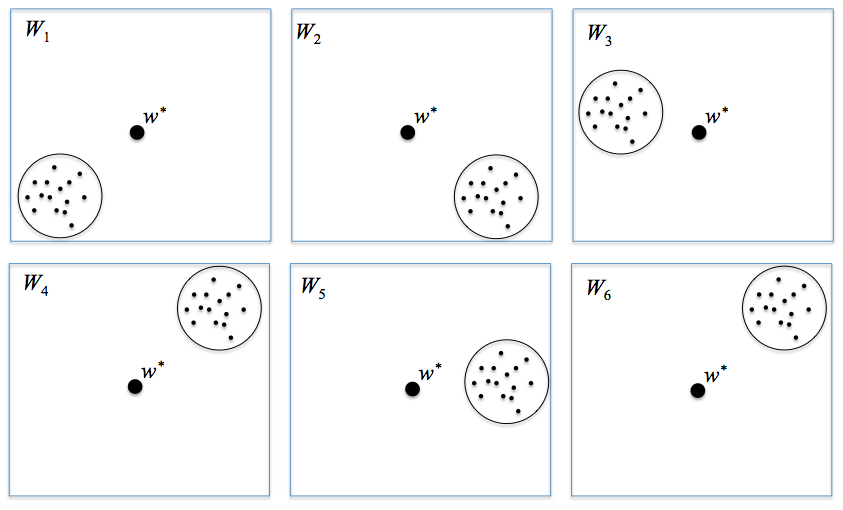
\includegraphics[width=.9\textwidth]{convexCombExample.png}
    \caption{A convex combination of $W_1,..., W_\gamma$ has high min and fuzzy min-entropy, but sketching by using the component flat distributions removes all entropy.}
\label{fig:convex comb}    
\end{figure}

\section{Proofs}
\subsection{Proof of \lemref{lem:fuzz necessary}}
\label{sec:proof fuzz necessary}
\begin{proof}
Let $W$ be a distribution where $\Hfuzz(W) = \Theta(\log n)$.  This means that there exists a point $m^*\in \mathcal{M}$ such that $\Pr_{w\in W}[\dis (w, m^*)\leq t] \geq 1/\poly(n)$.  Consider the following distinguisher $D$~(note that $D$ only provides an input and looks at the output, thus this distinguisher extends to the interactive setting):
\begin{itemize}
\item Input $r, p$.
\item If $\rep(m^*, p) = r$, output $1$.
\item Else output $0$.
\end{itemize}
First note that $|D|$ is of size $\max |\mathcal{M}|+ |\rep|$.  Clearly, $\Pr[D(R, P) = 1]\geq 1/\poly(n) - \delta$, while $\Pr[D(U_\kappa, P)=1 ]= 1/2^{-\kappa}$.  Thus, when $\kappa = \omega(\log n)$:
\[
\delta^D((R, P), (U_\kappa, P))\geq \frac{1}{\poly(n)} -\delta -  \frac{1}{2^{-\kappa}} = 1/\poly(n).
\]
\end{proof}

\subsection{Proof of \lemref{lem:flat hashing}}
\label{sec:proof of flat hashing}
\begin{proof}
We first argue security.  Fix some $W\in\mathcal{W}$. Since $\mathcal{K}$ and $W$ are independent $\Hav(W | \mathcal{K}) = \Hoo(W) = m$.  Then by \cite[Lemma 2.2b]{DBLP:journals/siamcomp/DodisORS08}, $\Hav(W | \mathcal{K}, F(K, W)) \ge \Hoo(W) - \log |F(K, W)| \ge m - \log |R|$.

We now argue correctness.  Fix some $w, w'$.  Let $W^*$ denote the set of elements in $W$ within distance $t$ of $w'$ recall that the size of $W^*$ is at most $B_{t, max}$ and since $w, w'$ are chosen independently of $\sketch$ this set is independent of the choice of $\mathcal{K}$.  Note $\rec$ will never output $\perp$ as the correct $w$ will match the hash, our goal is to bound the probability that another element $w^*$ collides, that is $F(K, w^*) = F(K, w)$.
\begin{align*}
\Pr[\exists w^* \in W^* |w^* \neq w \wedge F(K, w^*) = F(K, w)] &\le \sum_{w^*\in W^* | w^*\neq w} \Pr[F(K, w^*) = F(K, w)] \\
 &= \sum_{w^*\in W^* | w^*\neq w} \frac{1}{|R|} \le \frac{|B_{t, max}|-1}{|R|}
\end{align*}
Where the inequality proceeds by union bound, the first equality proceeds by the universality of $F$, and the second inequality proceeds by noting the number of neighbors is bounded by $|B_{t, max}|-1$.  This completes the proof.
\end{proof}

\subsection{Proof of \thref{thm:layered hashing}}
\label{sec:proof of layered hashing}
\begin{proof}
\textbf{Correctness:}  We begin by arguing correctness.  Let $\ell$ be a parameter describing the number of levels.\footnote{later we will set $\ell = m$ to simplify expressions and obtain the theorem statement.  The proof can be carried out for an arbitrary $\ell$.}  Fix some $w, w'$.  If $\Pr[W=w]\le 2^{-(n+\ell)}$, then $w$ is simply transmitted to $\rec$ and correctness is clear.  Now consider the case when $\Pr[W=w]> 2^{-(n+\ell)}$, let $L_i^*$ be the level of $\Pr[W=w]$.
Let $W^*$ denote the set of elements in $W$ within distance $t$ of $w'$ such that $\forall w \in W^*, \Pr[W^*=w]\in L_i^*$. The size of $W^*$ is at most $B_{t, i, max}$. The choice of $w, w'$ is independent of $\sketch$, so this set is independent of $\mathcal{K}_i$~(it does effect the value of $i$ but not the particular outcome from $\mathcal{K}_i$).  Note $\rec$ will never output $\perp$ as the correct $w$ will match the hash.  The probability that another element $w^*$ is:
\begin{align*}
\Pr[\exists w^* \in W^* |w^* \neq w \wedge F(K, w^*) = F(K, w)] &\le \sum_{w^*\in W^* | w^*\neq w} \Pr[F(K, w^*) = F(K, w)] \\
 &= \sum_{w^*\in W^* | w^*\neq w} \frac{1}{|R_i|} \le \frac{|B_{t, i, max}|-1}{|R_i|} = \delta
\end{align*}
Where the inequality proceeds by union bound, the first equality proceeds by the universality of $F$, and the second inequality proceeds by noting the number of neighbors is bounded by $|B_{t, i, max}|$.  

\textbf{Ideal Adversary with access to Level Information:} Before arguing security of the actual construction, we consider the optimum performance of an adversary that receives the level information.  %We first consider the optimum strategy for an adversary that receives just the information about the probability of $w$.  
An adversary that receives $i$ as input the best strategy is to guess a point that has the most nearby weight in that layer.  That is, $w^*\leftarrow A(i)$ such that $\max_{w^* \in \mathcal{M}}\Pr_{w\in W | 2^{-(i+1)}\le \Pr[W=w]\le 2^{-i}}[\dis(w, w^*)]$.The success of this adversary is at least $2^{-(i+1)}|B_{t,i, max}|$ as there at $B_{t, i, max}$ nearby points in that layer each with probability at least $2^{-(i+1)}$.  Note there are $n-m+\ell$ outcomes for $i$ so the overall success of such an adversary is at most $n-m+\ell$ better than an adversary without such input~(by~\cite[Lemma 2.2]{DBLP:journals/siamcomp/DodisORS08}).  That is, 
\begin{align}
\expe_{i | m\le i \le n+\ell}2^{-(i+1)}|B_{t, i, max}|&\le \expe_{i | m\le i \le n+\ell}\left( \max_{w^*\in W}\sum_{w\in W| 2^{-(i+1)}\le \Pr[W=w]\le 2^{-i} \wedge \dis(w, w^*) \le t}\Pr [W=w]\right) \label{eq:link fuzz 1}\\
&\le \left(n-m+\ell\right)\left(\max_{w^*\in W} \sum_{w\in W | \dis(w, w^*)\le t} \Pr[W=w]\right)\label{eq:link fuzz 2}\\
&= \left(n-m+\ell\right)\Hfuzz(W)\label{eq:link fuzz 3}
\end{align}
\textbf{Security:}
We now argue security.  First note that the total weight of points whose probability is less than $2^{-(n+\ell)}$ is at most $2^{-\ell}$~(there are at most $2^n$ points in the distribution).  That is, $\sum_{w | \Pr[W=w]\le 2^{-(n+\ell)}}\Pr[W = w] \le 2^{-\ell}$.  Let $1_{\text{low}}$ be the indicator random variable for $\Pr[W=w]\le 2^{-n}$.  Then 
\begin{align*}
\Hav(W | \sketch(W)) = -\log \left(\Pr[1_{\text{low}}=1] * 1 + \Pr[1_{\text{low}} =0]   2^{-\Hav(W | \sketch(W) \wedge 1_{\text{low}} = 0)}\right)\\
-\log\left( 2^{-\ell} + (1-2^{-\ell})2^{-\Hav(W | \sketch(W) \wedge 1_{\text{low}} = 0)}\right)
\end{align*}
For the remainder of the proof, we seek a bound on 
\[
2^{-\Hav(W | \sketch(W) \wedge 1_{\text{low}} =0} = \max_{w\in W | \Pr[W=w]>2^{-(n+\ell)}}\Pr[W=w | \sketch(W)].
\]
We separate out this quantity into levels:
\begin{align*}
\max_{w\in W | \Pr[W=w]>2^{-(n+\ell)}}\left(\Pr[W=w | \sketch(W)]\right) &= \expe_{i | m\le i \le n+\ell} \left(\max_{w\in W | \Pr[W=w]\in L_i} \Pr[W=w | \sketch(W), i]\right)\\
&= \expe_{i | m\le i \le n+\ell} \left(\max_{w\in W | \Pr[W=w]\in L_i} \Pr[W=w]*2^{|\sketch(W)|i|}\right)\\
&\le \expe_{i | m\le i \le n+\ell} \left(\max_{w\in W | \Pr[W=w]\in L_i} \Pr[W=w]*2^{H_0(\sketch(W) | i)}\right)\\
&\le \expe_{i | m\le i \le n+\ell} \left(2^{-i}*|B_{t, i, max}|/\delta\right)\\
&\le\frac{ \expe_{i | m\le i \le n+\ell} \left(2^{-(i+1)}*|B_{t, i, max}|\right)}{2\delta}\\
%&=\delta \sum_{i | m\le i \le n+\ell} \Pr[W\in L_i]\left(2^{-i}*|B_{t, i, max}|\right)
%\end{align*}
%Now consider This allows us to conclude that 
%\begin{align*}
%\max_{w\in W | \Pr[W=w]>2^{-n}\epsilon}\left(\Pr[W=w | \sketch(W)]\right) 
&= \frac{(n-m+\ell) 2^{-\Hfuzz(W)}}{2\delta}.
\end{align*}
Where the last line follows by Equations~\eqref{eq:link fuzz 1}-\eqref{eq:link fuzz 3}.
Combining both cases we have:
\begin{align*}
\Hav(W | \sketch(W)) = -\log \left(2^{-\ell}+\frac{(1-2^{-\ell})(n-m+\ell)2^{-\Hfuzz(W)}}{2\delta}\right).
\end{align*}
Setting $\ell = m$ yields
\begin{align*}
\Hav(W | \sketch(W)) &= -\log \left(m+\frac{(1-2^{-m})(n)2^{-\Hfuzz(W)}}{2\delta}\right)\\
&\ge -\log \min\{m, \frac{(1-2^{-m}) n2^{-\Hfuzz(W)}}{2\delta}\})-1\\
&\ge \Hfuzz(W) - \log n + \log \delta - \log (1-2^{-m}) - 2\\
&\ge \Hfuzz(W) - \log n + \log \delta - 3\\
\end{align*}
Where the third line follows from the second because $\Hfuzz(W)\le \Hoo(W) = m$. The last line follows from the fourth because if $m\ge 1$ then $\log (1-2^{-m})\le 1$ and if $m< 1$ the entire bound is vacuous as $\Hfuzz(W)< 1$.
\end{proof}

\section{Proof of \thref{thm:imposs sketch}}
\label{sec:proof secure sketch imposs}
\begin{proposition} 
\label{prop:each element good} For each $W\in\mathcal{V}$, $\Hfuzz(W) = \omega(\log n)$.
\end{proposition}
\begin{proof}
Consider some fixed $W\in\mathcal{V}$.  The value $w_1$ is uniform in a field of size $\omega(\poly(n))$, so $\Hoo(W) =\omega(\log n)$.  Recall that $t< \gamma$.  We now show that for any $w, w'\in W$, $\dis(w, w') = \gamma$ and thus $\Hfuzz(W) = \Hoo(W)$.  Fix some $w, w'\in W$.  Clearly, $w_1 \neq w_1'$, for any $i$, $w_i = a_i w_1 + b_i$ and $w_i' = a_i w_1' + b_i$.  Since $a_i\neq 0$, $a_iw_1 \neq a_iw_1'$ and thus $a_iw_1+b_i \neq a_iw_1'+b_i$.  That is, $\dis (w, w')  =\gamma$.
\end{proof}

\begin{proposition}
\label{prop:distribution uniform} $V$ is the uniform distribution over $\mathbb{F}^\gamma$.
\end{proposition}
\begin{proof}
Consider some $w\in V$.  Then $w$ was drawn from some intermediate distribution $W$ with coefficients $a_2, b_2, ..., a_\gamma , b_\gamma$.  The value $w_1$ is uniformly random and $w_i$ are uniformly random since $b_2,..., b_\gamma$ are uniformly random.
\end{proof}
\begin{lemma}
\label{lem:secure sketch entropy loss}
Fix some $\sketch, \rec$ algorithm with error $\delta < 1/4$, then $\tilde{H}_0(V | \sketch(V)) \le (\gamma-t+1)\log |\mathbb{F}|+1$.\footnote{This result is an extension of lower bounds from~\cite[Appendix C]{DBLP:journals/siamcomp/DodisORS08}.  Dealing with imperfect correctness makes the bound more complicated.  In particular, we can only argue about the average remaining support size.}
\end{lemma}
\begin{proof}
We assume that $\rec$ is deterministic in our analysis.  Any randomness necessary for the \rec algorithm can be provided by \sketch.  We do not consider these coins in our security analysis~(and thus, they can be considered private).
By the definition of correctness for $(\sketch, \rec)$, 
\[
\forall w, w', \Pr_{ss\leftarrow \sketch(w)} [\rec(w', ss) = w] >1-\delta.
\]
%For most $p$, $\rec$ works on most neighbors of $w$.  
Fix some $w$.  
By Markov's inequality, there exists a set $A_{ss}$ such that $\Pr[ss\in A_{ss}]\ge 1/2$ and $\forall ss\in A_{ss}$, 
\[
\{w' | \dis (w', w)\le t \wedge \rec(w', p) \neq w\}\le 2\delta < 1/2.\]

Consider some $ss^*\in A_{ss}$.  We now show that $H_0(V | \sketch(V) = ss^*) \le (\gamma-t+1)\log |\mathbb{F}|$.  Note for the true value $w$ sketched $\{w' | \dis(w, w') \le t \wedge \rec(w', p) \neq w] \le 2\delta$.  Thus for every value in $V|\sketch(V) = ss^*$ this is also true.  This makes the support of $V|\sketch(V)=ss^*$ a $(t, 2\delta)$-Shannon code~(see \defref{def:shannon-code}).  In particular, this implies that for all $w_1, w_2 \in V|\sketch(V)=ss^*$, $\dis(w_1, w_2)\ge t$~(since $2\delta< 1/2$).  That is $V|\sketch(V)=ss^*$ is a set with minimum distance at least $t$.  By the Singleton bound, this implies that $H_0(V |\sketch(V)=ss^*) \le (\gamma -t+1 )|\mathbb{F}|$.  Averaging over $\sketch(V)=ss^*$ one has that $\tilde{H}_0(V|P) \le (\gamma -t +1) \log|\mathbb{F}| +1$.
%By the Markov inequality, 
%\[
%\forall w, w^*, \Pr_{p \leftarrow \sketch(w)} [ \Pr[\rec(w^*, p) = w] \le 1-2\delta ] < \delta /2.
%\]
%That is, for most $p$, $\Pr[\rec(w^*, p) = w] > 1-2\delta>1/2$.
%
%Outline of what I want to say.
%\begin{itemize}
%\item Suppose we are at some good sketch value, that is, the sketch decodes well for $w^*$ close to the true value $w$.
%\item Then for the true value that was sketched, for most neighbors $w^*$ of $w$, $\Pr[\rec(w^*, p) =w] >1/2$.  
%\item For a value $w'$ to be in the support of $W | P=p$, it must be for all neighbors of $\Pr[\rec( w', p) =w ]>1/2$.
%\item This implies that if $w_1, w_2 \in W|P = p$, then $\dis (w_1, w_2)\ge t$.
%\item Conditioned on $P=p$, $W| P=p$ is a good code for random errors.
%Consider some subset $G\subseteq supp(W| P=p)$ with $\Pr (W| P=p \in G)\ge 1/2$.  Then for all $w\in G$ the probability they recover correctly is at least $1-4\delta$~(by another application of Markov).  
%\item This, means that the size of $|G|$ is at most $n -\log |B_t|$.
%\end{itemize}
\end{proof}
We showed that for most values of $\sketch$ many values of $V$ are removed from the support.  We now show that the information contained in $Z$ is enough to nearly determine the actual sketched value.

\begin{lemma}
\label{lem:side info determines sketch}
$\Hav(V | \sketch(V), Z) \le \Theta(1)$.
\end{lemma}
\begin{proof}
Recall that $Z$ consists of $2\gamma$ coefficients and there are $(|\mathbb{F}|-1)^{\gamma-1} |\mathbb{F}|^{\gamma-1}$ equally likely values for $Z$.
 As described above, the view of $\sketch, \rec$ is a uniform distribution $V$.  We know show there are many possible values for $Z$.  The only information seen by $\sketch$ algorithm is in the point $V=v$.  The length of this point is $|\mathbb{F}|^\gamma$.  Conditioned on this information there are still many possible values for $Z$.  That is, 
 \[
 \forall v, H_0(Z | V=v) =\log \left(\frac{(|\mathbb{F}|-1)^{\gamma-1} |\mathbb{F}|^{\gamma-1}}{|\mathbb{F}|^\gamma}\right) = \log \left( (|\mathbb{F}|-1)^{\gamma-1}/|\mathbb{F}|\right).
 \]
Consider two possible $z_1, z_2$ that are possible values of $Z$.  The distributions $V| Z=z_1$ and $V | Z=z_2$ intersect at one point~(namely $v$).  

We now show for any sketch algorithm, for possible values of $Z$ conditioned on $V=v$ there are few points included in the support of $V |\sketch(V)$.  For any two values of $z_1, z_2$ the distributions $V| Z= z_1$ and $V | Z=z_2$ intersect at most one point.  The distributions $V | Z=z_1$ and $V| Z=z_2$ for possible $z_1, z_2$~(having seen $v$) overlap only at the point $v$.  This means for any $v^*\in V| \sketch(V)$ (other than the true $v$) there is at most one $z$ such that $v^*\in V | \sketch(V), Z=z$.  Thus, we ask The optimum strategy is to include these values uniformly from different $Z$ values.

We show this across different sketch values.  Consider some fixed sketch value $s$ and let $h_s \overset{def}= H_0(V | \sketch(V) = s)$.  That is, there are $2^{h_s}$ possible values for $V$ conditioned on $\sketch(V) = s$.  Furthermore, recall that 
\[
\log \expe_{s\in \sketch(V)} 2^{h_s} = \log \expe_{s\in \sketch(V)} 2^{H_0(V | \sketch(V) = s)}  = \tilde{H}_0(V | \sketch(V)) %\le   (\gamma-t+1)\log |\mathbb{F}|+1.
\]  
Conditioned on seeing the point $V$ there are $(|\mathbb{F}|-1)^{\gamma-1}/|\mathbb{F}|$ possible values for $Z$ with disjoint support outside of the sketched point.  Consider these possible values for $Z$ as bins to be filled with the $2^{h_{ss}}$ balls~(possible values of $V | \sketch(V)=ss$).  The average number of balls in each bin is maximized when the bins are filled equally.  That is, the average number of balls in each bin is bounded by the number of balls divided by the number of bins.  That is, 
\begin{align*}
\tilde{H}_0(V |Z  , \sketch(V) = ss) &\le \log \left(\frac{\text{\# bins}}{\text{\# balls}}\right)\\
&= \log \left(\frac{2^{h_{ss}}|\mathbb{F}|}{(|\mathbb{F}|-1)^{\gamma-1}} \right)
\end{align*}
Then averaging over the possible values of $s$, we have the following as long as $t\ge 4$:
\begin{align*}
\tilde{H}_0(V |Z , \sketch(V) ) &= \log \expe_{s\in \sketch(V)} 2^{\tilde{H}_0(V |  \sketch(V) =ss , (Z| \sketch(V) =ss) )}\\
&= \log\expe_{s\in \sketch(V)} \left(\frac{2^{h_s}|\mathbb{F}|}{(|\mathbb{F}|-1)^{\gamma-1}} \right)\\
&= \log \frac{|\mathbb{F}|}{(|\mathbb{F}|-1)^{\gamma-1}} \expe_{s\in \sketch(V)} 2^{h_s}\\
&=\log |\mathbb{F}| - (\gamma -1)\log (|\mathbb{F}|-1) + \log \expe_{s\in \sketch(V)} 2^{h_s}\\
&=\log |\mathbb{F}| - (\gamma -1)\log (|\mathbb{F}|-1) + \tilde{H}_0(V | \sketch(V))\\ 
&\le \log |\mathbb{F}| - (\gamma -1)\log (|\mathbb{F}|-1) + (\gamma-t+1)\log |\mathbb{F}|+1\\
&\le (\gamma-t+2)\log |\mathbb{F}| - (\gamma-1) \log (|\mathbb{F}|-1)+1\\
&< (\gamma-t+2)\log |\mathbb{F}| - (\gamma-2) \log |\mathbb{F}| +1 \ \ \ \ \mbox{(by \lemref{lem:log-minus-one})}\\
&\le (4-t)\log |\mathbb{F}| +1\\
& <1\,.
\end{align*}
\lnote{need for \lemref{lem:log-minus-one}:  $\gamma-1\le |F|$ and $|F|\ge 4$}
\lnote{change the any needed theorem statements it affects in light of the tightening}

\lnote{this lemma should probably live elsewhere since it is also needed for the FE case}
\bnote{fine with it being here as the FE case lives in the appendix too}
\begin{lemma}
\label{lem:log-minus-one}
For any real numbers $\alpha \leq \beta$ with $\beta \ge e+1$ (in particular, $b\ge 4$ suffices), the following holds:
$\alpha \log (\beta-1) > (\alpha-1)\log \beta$. 
\end{lemma}

\begin{proof}
Because $\beta-1$ is positive, and $1+x<e^x$ for positive $x$,
$$1+\frac{1}{\beta-1} < e^{\frac{1}{\beta -1}}\,.$$  Therefore, 
$$\left(1+\frac{1}{\beta-1}\right)^{\alpha-1} < e^{\frac{\alpha-1}{\beta-1}}\le e < \beta-1$$ (since $\alpha\le \beta$). Multiplying both sides by $(\beta-1)^{\alpha-1}$, we obtain
$$\beta^{\alpha-1} < (\beta-1)^\alpha\,.$$
Taking the logarithm of both sides, we get the desired result.
\end{proof}

 \end{proof}
\noindent \thref{thm:imposs sketch} follows using the change of quantifiers in \corref{cor:no fuzz for dist}.


\section{Proof of \thref{thm:imposs fuzz ext}}
\label{sec:fuzz ext proof}
\begin{proposition} 
\label{prop:dist fuzzy ent fuzz}
For each $W\in\mathcal{V}$, $\Hfuzz(W) = \omega(\log n)$.
\end{proposition}
\begin{proof}
Consider some fixed $W\in\mathcal{V}$.  The value $w_{1,..., \nu}$ is uniform, so $\Hoo(W) =\omega(\log n)$.  Recall that $t=o (n/\nu)$.  We now show that for any $w, w'\in W$, $\dis(w, w') \ge n/\nu$ and thus $\Hfuzz(W) = \Hoo(W)$.  Fix some $w, w'\in W$.  Denote by $x, x'$ the values that produce $w, w'$ respectively.  Clearly, $x\neq x'$.  Thus, for any $i$, $a_i w_1 + b_i \neq a_i x' + b_i$.  This implies that $w_{i\nu+1,...., (i+1)\nu} \neq w'_{i\nu+1,..., (i+1)\nu}$ and thus $\dis(w, w') \ge n/\nu$.  Thus, $\Hfuzz(W) = \Hoo(W)= \omega(\log n)$.
\end{proof}

\begin{proposition}\label{prop:dist uniform fuzz}
$V$ is the uniform distribution over $\mathbb{F}^\gamma$.
\end{proposition}
\begin{proof}
Consider some $w\in V$.  Then $w$ was drawn from some intermediate distribution $W$ with coefficients $a_2, b_2, ..., a_\gamma , b_\gamma$.  The value $w_{1,...,\nu} =x $ is uniformly random and $w_{i\nu+1,...,(i+1)\nu}$ are uniformly random since $b_2,..., b_\gamma$ are uniformly random.
\end{proof}

The previous two propositions were similar to the secure sketch case.  The remainder of the proof is significantly different.  We show for any $(\gen, \rep)$ many keys have few possible values that could produce them in the metric space once $p$ is published.  Then an adversary that sees $z$ is able to eliminate many possible keys and thus effectively distinguish the key from random.

\begin{lemma}
\label{lem:fuzz can't get key}
Fix some $(\gen, \rep)$ algorithm with $\kappa \ge 1$.  There exists an information-theoretic distinguisher between $(R, P, Z)$ and $(U_\kappa, P, Z)$ with advantage $\epsilon = 1/4-\ngl(n)$.
\end{lemma}
\begin{proof}
We assume that $\rep$ is deterministic in our analysis.  Any randomness necessary for the \rep algorithm can be provided by $\gen$.  We do not consider these coins in our security analysis~(and thus, they can be considered private).  Denote by $(R, P) \leftarrow \gen(V)$.

%By the definition of correctness for $(\sketch, \rec)$, 
%\[
%\forall w, w', \Pr_{p\leftarrow \sketch(w)} [\rec(w', p) = w] >1-\delta.
%\]
%For most $p$, $\rec$ works on most neighbors of $w$.  
%Fix some $w$.  
By Markov's inequality, there exists a set $A_{p}$ such that $\Pr[p\in A_{p}]\ge 1/2$ and $\forall p\in A_{p}$, 
\[
(R |P =p, P = p ) \approx_{2\epsilon} (U_\kappa , P =p).
\]
%\{w' | \dis (w', w)\le t \wedge \rec(w', p) \neq w\}\le 2\delta < 1/2.\]

Consider some $p^*\in A_{p}$.  %Since $(R | P=p^*, p^*)\approx_{2\epsilon} (U, p^*)$ this means that $R|P=p^*$ is at least $(1-2\epsilon)2^\kappa$.  
The distribution $R|P=p^*$ is the set of possible keys.
The distribution $R|P=p^*$ induces a partition on the metric space.  That is, for every $w\in\mathcal{M}$, there exists a unique value $r$ such that $\rep(w, p^*) =r$.  Denote this partition by $Q_{p^*,r} = \{w | \rep(w, p^*) = r\}$.  

Many of these sets must be small.  That is, there exists a set $R_{small}$  where $|R_{small} | \ge 2^{\kappa-1}$ such that for all $r\in R_{small}$,  $|Q_{p^*, r}|\le \mathcal{M}/2^{\kappa-1} = 2^{n-\kappa +1}$.  If not, there exists a set of $r$ of size $2^{\kappa-1}$ that all have at least $\mathcal{M}/2^{\kappa-1}$ points.\footnote{In the case where $\kappa=1$, $R_{small}$ still has at least one element.}  This is more points than exist in the metric space.  

For the remainder of the proof we restrict ourselves to elements in $R_{small}$.  We first define the interior of a set:%Define two sets, called the interior and crust respectively: \bnote{change term crust?}
\begin{align*}
\inter(Q_{p^*, r}) = \{w | \rep(w, p^*) = r \wedge \forall w', \dis(w, w') \le t \wedge \rep(w', p^*) =r\},\\
%\crust(Q_{p^*, r}) = \{w | \rep(w, p^*) = r \wedge \exists w', \dis(w, w')\le t \wedge \rep(w', p^*) \neq r\}.
\end{align*}

%Note that $\crust(Q_{p^*, r}) \cap \inter(Q_{p^*,r}) =\emptyset$.  
We now show that for $r\in R_{small}$ there are few points in $\inter(Q_{p^*, r})$.  Consider some $r^*\in R_{small}$.  We will use the term deficient sphere:
\begin{definition}
A set $S$ is a $\beta$-deficient ball if there exists a point $x$ such that $B_{\beta-1}(x) \subseteq S \subseteq B_{\beta}(x)$.
\end{definition}

We now proceed to show that the interior of each $Q_{p^*, r^*}$ is small~(using the isoperimetric inequality on the Hamming space):
%Recall that $B_{n-\kappa-t}$ denotes the ball of radius $n-\kappa -t$.

\begin{lemma}
$|\inter(Q_{p^*, r^*})| \le 2^{n-4\nu}$.
\end{lemma}
\begin{proof}
By the isoperimetric inequality on the Hamming space~(we use a version due to~\cite[Theorem 1]{frankl1981short}, the original result is due to Harper~\cite{harper1966optimal})\bnote{better citation?}, there exists a $\beta$-deficient ball $S_{p^*, r^*}$ centered at $0$ and a set $D$ such that $|S_{p^*, r^*}| = |\inter(Q_{p^*, r^*})|$, $|D| = |Q_{p^*, r^*}^\complement|$ and $\forall s\in S_{p^*, r^*}, d\in D$, $\dis(s, d) \ge t$~(alternatively, the distance between the sets is $t$).  Furthermore, note that $S_{p^*, r^*} \cup D$ is a deficient ball~(and its radius is $t$ larger than $S_{p^*, r^*}$).
We now find the size of $S_{p^*, r^*}$.

Recall that $|S_{p^*, r^*} \cup D| = |Q_{p^*, r^*} | \le 2^{n-(\kappa-1)}\leq |\mathcal{M}|/2$.  Since this set contains less than half the points in the metric space we know its radius at most $n/2$.  This means that $|S_{p^*, r^*}|$ is a deficient sphere of radius at most $n/2-t$.  Let $X$ denote a uniform string on $\zo^n$.  We use Hoeffding's inequality~\cite{hoeffding1963probability}:

\begin{align*}
|S_{p^*, r^*}| \le \{ x | \dis (x, 0)\le n-t\} &= 2^n \Pr[ wt(X) \le (1/2-t/n)n] \le 2^n e^{-n ((t/n)^2)} = 2^n e^{-4\nu} \le 2^{n - 4\nu}
\end{align*}
% That is, We now find the maximum radius ball that contains at most $2^{n-(\kappa-1)}$ points.  That is, $\max \{d\in \mathbb{Z^+}| B_d \le 2^{n-(\kappa-1)}\}$.  Recall that $2^{n-(\kappa-1)} \ge |B_d| \ge (n/d)^d$\bnote{this bounds sucks! do better}.  Thus,
%\[n-(\kappa-1) \ge d (\log n - \log d).\]  
%We first show that $d\le n/2$.  Since $|S_{p^*, r^*} | \le 2^{n-(\kappa-1)}/2^n \le 1/2$, then $d\le \lceil n/2\rceil$.  This is because $\sum_{i=0}^{\lceil n/2 \rceil} {n\choose i} \ge 2^{n-1}$.  
%
%Since $d\le 1/2$, $d\le d(\log n - \log d)$ and thus: $d\le n-(\kappa+1)$.  That is, $S_{p^*, r^*} \cup D$ is a deficient sphere of radius at most $n-(\kappa-1)$.  This means that $S_{p^*, r^*}$ is a deficient sphere of radius at most $n-(\kappa-1)-t$.  That is $S_{p^*, r^*}$ is contained in a sphere of radius $n-\kappa-t+2$. And thus, $|\inter(Q_{p^*, r^*}|\le |B_{n-\kappa-t+2}|$.\bnote{we need a much better bound here.  This is a radius of almost $n$}
\end{proof}

We have shown that $|\inter(Q_{p^*, r^*})| \le 2^{n-4\nu}$.  %Define the set $K_{bad} = \cup_{r^*\in R_{small}} |Q_{p^*, r^*}|$ and note that $|K_{bad} | \le  |B_{n-\kappa -t+2}||R_{small}|$.
To complete the proof it suffices to show that for most values of the auxiliary information $Z$ there are many parts $Q_{p^*, r^*}$ that do not receive any points.  
Recall that $Z$ consists of $2n/\nu$ coefficients and there are $(2^t-1)^{\nu-1} 2^{n-\nu}$ equally likely values for $Z$.
 As described above, the view of $\gen, \rep$ is a uniform distribution $V$.  We know show there are many possible values for $Z |P=p^*$.  The only information about $Z$ is contained in the point  $V=v$.  The length of this point is $2^n$.  Conditioned on this information there are still many possible values for $Z$.  That is, 
 \[
 \forall v, H_0(Z | V=v) =\log \left(\frac{(2^{n/\nu}-1)^{\nu-1} 2^{n-\nu}}{2^n} \right) = \log \frac{(2^{n/\nu}-1)^{\nu-1}}{2^{\nu}} >\log  \frac{(2^{n/\nu})^{\nu-2}}{2^{\nu}}  \log \frac{2^{(n-2\nu))}}{2^\nu} = n -3\nu.
 \]
 where the inequality follows by \lemref{lem:log-minus-one}.
Consider two possible $z_1, z_2$ that are possible values of $Z$.  The distributions $V| Z=z_1$ and $V | Z=z_2$ intersect at one point~(namely $v$).  

This means that the $\gen$ algorithm may include points for possible $Z$ values into parts $Q_{p^*, r^*}$~(other than $v$) and these values are disjoint.  The optimum strategy is to include these values uniformly from different $Z$ values.  Consider the set of $r^*$ with small support, that is $Q_{small} = \cup_{r\in R_{small}} \inter(Q_{r, p^*})$.  Note that $Q_{small} \le 2^{n-n^{1/3}}|R_{small}|$.
That is, 
\begin{align*}
\expe_z |Q_{small} \cap V | P=p^* \wedge Z=z | &\le \frac{2^{n-4\nu}|R_{small}|}{2^{n - 3\nu}}\\
&=\frac{|R_{small}|}{2^{\nu}}.
\end{align*}
Thus, at most $1/2^{\nu} = \ngl(n)$ fraction of keys in $R_{small}$ have any support  conditioned on $p^*$ and $Z$~(note this is an expectation across the values of $Z$).  We now present a distinguisher $D_{p^*}$ for a particular $p^*$:
\begin{enumerate}
\item On input $x, z$.
%\item If $x\not \in R_{small}$ output random bit $b$.
\item Compute $V|P=p^* \wedge Z=z$ and $Q_{p^*, x}$. 
\item If $(Q_{p^*, x} \cap V|P=p^* \wedge Z=z) =\emptyset$ output $b=0$.
\item Else output $b=1$.
\end{enumerate}

The distinguisher $D(x, p, z)$ is formed by calling $D_p(x, z)$ when $p\in A_p$ and outputting a random bit otherwise.  The advantage of $D$ is 
\begin{align*}
\Pr[D(R, P, Z) = 1] &- \Pr[D(U, P, Z) =1]=(\Pr[D(R, P, Z) = 1| P\in A_p] - \Pr[D(U, P, Z) =1 | P\in A_p])\Pr[P\in A_p]\\
&\ge \sum_{p^*\in A_p} \Pr[P=p^*] \left(1 - \Pr[D_{p^*}(U, Z)=1]\right)\\
&\ge \sum_{p^*\in A_p} \Pr[P=p^*] \left(1- \Pr[D_{p^*}(U, Z)=1 | U\in R_{small}]\Pr[U\in R_{small}] - \Pr[U\not\in R_{small}]\right)\\
&\ge \sum_{p^* \in A_p} \Pr[P=p^*]\left(1/2-\ngl(n)\right) = 1/4-\ngl(n).
\end{align*}
The fourth line follows since $R_{small} \ge 2^{\kappa-1}$ and thus $\Pr[U\in R_{small}]\ge 1/2$.  The last line follows by recalling that $\Pr[P\in A_p]\ge 1/2$.
%We now show that $\expe | Q_{p^*, r^*} \cap V | P=p^* \wedge Z=z| \le (1- \epsilon) |R_{small}|$. 
%We use the combinatorial bound that $|B_d| \le \left(\frac{ne}{d}\right)^d$ \bnote{this bound is terrible!}.  We then have that, 
%\begin{align*}
%\expe_z |K_{bad} \cap V | P=p^* \wedge Z=z | &\le \frac{|B_{n-\kappa -t+2}||R_{small}|}{2^{n\nu -n -2\nu +1}}\\
%&\le  \frac{\left(\frac{ne}{n-\kappa -t+2}\right)^{n-\kappa -t+2}}{2^{n\nu -n-2\nu+1}}|R_{small}|\\
%&\le \frac{2^{3(n-\kappa -t +2)}}{2^{n -n/\nu-2\nu+1}}|R_{small}|
%%&= \frac{\left(2^{\log n+ \log e - \log (n-\kappa -t+2)}\right)^{n-\kappa -t+2}}{2^{n\nu -n-2\nu+1}}|R_{small}|\\
%%&=2^{(n-\kappa-t+2)(\log n+ \log e - \log (n-\kappa -t+2)) - (n\nu -n 2\nu+1)} |R_{small}|
%\end{align*}
%\bnote{the two combinatorial bounds we are using aren't good enough}
%To show that $\epsilon \ge 1/2$ we have that 
%%\begin{align*}
%%(n-\kappa-t+2)(\log n+ \log e - \log (n-\kappa -t+2)) - (n -n/\nu- 2\nu+1) 
%%\end{align*}
%\bnote{why was that sufficient to break security}
%\bnote{still working this isn't complete}

This completes the proof of \lemref{lem:fuzz can't get key}.
\end{proof}



%\section{Coding Theory}
%\begin{definition}
%\label{def:shannon-code}
%Let $\mathcal{C}$ be a set over space $\mathcal{M}$.  We say that $\mathcal{C}$ is an $(t,\epsilon)$-\emph{Shannon code} if there exists an efficient procedure $\rec$ such that for all $c\in \mathcal{C}$, $\Pr_{w' | \dis(w', w)\le t}[\rec(c') \neq c]\le \epsilon$. To distinguish it from the average-error Shannon code defined below, we will sometimes call it \emph{maximal-error} Shannon code.
%\end{definition}
%
%
% \begin{definition}
%Let $C$ be a distribution over space $\mathcal{M}$.  We say that $C$ is an $(t,\epsilon)$-\emph{average error Shannon code} if there exists an efficient procedure $\rec$ such that for all $t'\le t$
%$\Pr_{c\leftarrow C}[\rec(\neigh(c, t')) \neq c]\le \epsilon$.
%\end{definition}
%An average error Shannon code is one whose average probability of error is bounded by $\epsilon$.  See~\cite[Pages 192-194]{cover2006elements} for definitions of average and maximal error probability.  An average-error Shannon code is convertible to a maximal-error Shannon code with a small loss.  We use the following pruning argument from~\cite[Pages 202-204]{cover2006elements} %(we provide a proof in \secref{sec:proof of average to maximal error}):
%\begin{lemma}
%\label{lem:averageToMaximalError}
%Let $C$ be a $(t, \epsilon)$-average error Shannon code with recovery procedure $\rec$ such that $\Hoo(C)\geq k$.  There is a set $\mathcal{C}'$ with $|\mathcal{C}'|\ge2^{k-1}$ that  is a $(t, 2\epsilon)$-(maximal error) Shannon code with recovery procedure $\rec$.
%\end{lemma}
%
%\bnote{This comes from asiacrypt paper, what to cite?}
%\section{Block Unguessable Distributions}
%\begin{definition}~\cite[Definition 4.2]{canetti2014key}
%\label{def:block guessable}
%Let $I_w (\cdot, \cdot)$ be an oracle that returns \[I_w(j, w_j')=
%\begin{cases}
%1 & w_j = w_j'\\
%0 & \text{otherwise}.
%\end{cases}
%\]
%A source $W = W_1||...|W_\gamma$ is a $(q, \alpha, \beta)$-\emph{unguessable block distribution} if there exists a set $J\subset\{1,..., \gamma\}$ of size at least $\gamma -\beta$ such that for any unbounded adversary $S$ with oracle access to $I_w$ making at most $q$ queries
%\[
%\forall j\in J, \Hav(W_j |View(S^{I_{W}(\cdot, \cdot)}))\geq \alpha.
%\]
%\end{definition}

\section{Old Proofs}
\bnote{I don't think we need anything from these sections}
\subsection{Flat Sources with Sketches that Write a Fixed Number of Bits}
We begin by trying to remove the restriction that every point in the metric space has a fixed number of neighbors in a distribution.  We start with sketches that write down a fixed number of bits~(independent of their input $w$).   We will show a lower bound on the number of bits that a $\sketch$ algorithm must write down.  We assume that all coins of $\sketch$ are provided to $\rec$ and that $\rec$ is deterministic~(any coins needed for $\rec$ can be flipped by $\sketch$ in this model).

\begin{lemma}
Let $W$ be a flat distribution and let $(\sketch, \rec)$ be a secure sketch for $W$.  Let $W$ be a $(c, t)$-bounded neighbor distribution.  Let $S_{coin}$ be the number of sketches that can be produced by any fixing of $coin$.  Then the error $\delta$ of $(\sketch, \rec)$ is at least $\frac{\expe_{coins}L(coins)}{c}$.  
\end{lemma}
\begin{proof}
We consider a fixed $w'$ that has $c$ neighbors in the distribution.  We assume $\rec$ has access to all coins of $\sketch$.  Furthermore, we assume that $\rec$ is deterministic and that any coins necessary are provided by $\sketch$).  

Denote by $S_{coin, R}$ the set of possible sketches for a given set of coins on all values in $R$.  Furthermore, denote by $S_{coin}$ the set of possible sketches for all values $w$~(for a given value of coin) and note that $S_{coin, R} \subset S_{coin}$.  Then $\rec(\cdot, w', coin)$ must fail to recover $|R|-|S_{coin, R}|$ fraction of $w\in R$~(recalling that $\rec$ is deterministic for this fixing of $coin$).  This means that the total number of pairs $(w, coin)$ for which $\rec$ fails to recover is $2^{|coins|}R - \sum_{coins} |S_{coin, R}|$.

This means there must exist some $w$ such that the number of $coin$ values for which $\rec$ fails to recover is 
\[
2^{|coin|} - \frac{\sum_{coin} |S_{coin, R}|}{R}.
\]
 This means that for this $w$, 
\[
\Pr_{coin}[s \leftarrow \sketch(w, coin) \wedge w = \rec(s, w', coin)] < 1- \frac{\expe |S_{coin, R}|}{|R|} = 1-\frac{\expe |S_{coin, R}|}{c} \le 1-\frac{\expe |S_{coin}| }{c}.
\]

%Consider the function $\rec(w', ss, r)$ where $ss$ is the sketch produced by $\sketch(w)$ and $r$ are the coins used by $\sketch$.  
\end{proof}

For deterministic sketches:
\[
\Hav(W|S ) = -\log \left(\sum_{s\in S} \Pr[S = s] \frac{2^{-\Hoo(W)}}{\Pr[S=s]}\right) = -\log \left(2^{-\Hoo(W)} |S| \right)  = \Hoo(W) - H_0(S).
\]

\subsection{How many bits for distribution oblivious sketch} 
\begin{lemma}
Let $\mathcal{W}$ be the set of all $t_{cor}$-well spread distributions.  Let $t = \lfloor (t_{cor}-1)/2\rfloor$ and let $(\sketch, \rec)$ be a $(\mathcal{M}, m, \tilde{m}, t )$-secure sketch.  Then the average length of $\sketch$ is at least $\log |B_{t}|$.
\end{lemma}
\bnote{what do we mean by average here?  we mean when receiving a uniform input across the coins.  Maybe, there are distributions where it writes down a little.  What's the right thing to say?  Markov?}
\begin{proof}
Let $\mathcal{M}$ be a metric space.
Let $\mathcal{W}$ be the set of all $t_{cor}$-well spread distributions on $\mathcal{M}$.  
Consider the following experiment:
\[
W\leftarrow \mathcal{W} \wedge w \leftarrow W \wedge w'\leftarrow B_{t_{cor}}(w) \wedge ss \leftarrow \sketch(w) \wedge w^* \leftarrow \rec(w', ss).
\]
That is, the adversary uniformly samples a well-spread distribution and then a point from the well-spread distribution.  
Since $(\sketch, \rec)$ works for any well-spread distribution the $\Pr[w^* = w] =1 $ in the above experiment.   Denote by $X$ the joint distribution of $w, w'$ produced in the above experiment.  Now consider the following experiment
\[
v \leftarrow U_{\mathcal{M}} \wedge v'\leftarrow B_{t_{cor}}(v) \wedge ss \leftarrow \sketch(v) \wedge v^* \leftarrow \rec(v', ss).
\]
Denote by $Y$ the joint distribution of $v, v'$ produced in the above experiment.  Then $X\overset{d}= Y$.  That is, the view of $(\sketch, \rec)$ is identically distributed in both cases.  Thus, $\Pr[v^* = v] = 1$.  For the uniform distribution the entropy retained by a secure sketch is at most $\Hav(U_{\mathcal{M}} | \sketch(U_{\mathcal{M}})) \le \log |\mathcal{M}| - \log |B_t(\cdot)|$~\cite[Lemma C.1]{DBLP:journals/siamcomp/DodisORS08}.  For a secure sketch to lose $\log |B_t(\cdot)|$ bits of entropy it must write down at least $\log |B_t(\cdot)|$ bits on average~\cite[Lemma 2.2b]{DBLP:journals/siamcomp/DodisORS08}.  Thus, $(\sketch, \rec)$ writes down at least $\log |B_t(\cdot)|$ bits on the uniform distribution and its view is identical on $X$ so it writes down at least $\log |B_{t_{cor}}|$ bits on $X$.  This completes the proof.
\end{proof}
\noindent
\textbf{Notes:} In the above lemma, the relation between the well-spreadness of the class of distributions and the correctness of the fuzzy extractor is not important and is made to match the relation in \lemref{lem:nosketchwellspread} for convenience.  The bound is purely derived from the correctness condition, the well-spreadness of the distribution can essentially be arbitrarily replaced~(as long as the maximal distance point from any point in the metric space is the same).

Furthermore, the above lemma easily extends to the setting where the distributions are not well-spread as long as there is an adversary strategy of choosing the input distribution that produces an input to sketch that is identically distributed to the uniform distribution.

The above lemma only talks about how many bits the algorithms must write down.  It does not say that the entropy of the distribution must decrease~(this is the important question).  We now proceed to this question.



\end{document}











